\documentclass{mini}
\usepackage[utf8]{inputenc}
\usepackage{fancyvrb}
\usepackage{amsmath}
\usepackage{subfig}
\newcommand{\degree}{\ensuremath{^\circ}}
\newcommand{\hilight}[1]{\colorbox{yellow}{#1}}
\linespread{1.5}
\DeclareUnicodeCharacter{00A0}{~}

%------------------------------------------------------------------------------%
\title{Analiza możliwości wykorzystania w~algorytmie CMA-ES wiedzy o~ograniczeniach kostkowych}

\author{inż. Robert Jakubowski}
\supervisor{dr hab. inż. Jarosław Arabas prof. nzw. PW}
\type{magisters}
\monthyear{Maj 2016}
\date{\today}
\album{237545}
%------------------------------------------------------------------------------%
\begin{document}

\maketitle

\pagebreak
\thispagestyle{empty}

\openup -0.2em %make it fit on one page
\tableofcontents 
\openup 0.2em %make it fit on one page

\thispagestyle{empty}
\raggedbottom
\pagebreak


\section{Streszczenie}

\pagebreak

\section{Wstęp}

\subsection{Cel pracy}

\pagebreak

\section{Techniki uwzględniania ograniczeń}
Niektóre problemy optymalizacyjne posiadają ograniczenia. Szukając rozwiązania należy zapewnić, że rozwiązanie będzie dopuszczalne. Zgodnie z --------łącze-------- techniki, które w tym pomagają można podzielić w następujący sposób:
\begin{itemize}[noitemsep]
\item definicja przestrzeni przeszukiwań - zapewnienie, że podczas krzyżowań, mutacji i innych zmian punktów, żaden z punktów nie wypadnie poza przestrzeń przeszukiwań,
\item modyfikacja funkcji celu - zmienienie funkcji celu tak, aby funkcja celu dla punktów spoza ograniczeń zwracały gorsze wyniki,
\item transformacja rozwiązań - punkty, które są poza ograniczeniami zostają zamieniane na punkty, które znajdują się w ograniczeniach.
\end{itemize}

W tej pracy skupiono się na transformacji rozwiązań

\subsection{Transformacje rozwiązań} \label{transformacje}
Nie istnieje jedna technika transformacji rozwiązań spoza ograniczeń, na dopuszczalne. W kolejnych podrozdziałach opisane są metody transformacji rozwiązań, które były badane. Każda z technik jest opisana słownie oraz pseudokodem. Opis słowny zawiera wyjaśnienie, co się dzieje z punktem, który znalazł się poza ograniczeniem. W pseudokodzie zastosowane następujące oznaczenia:
\begin{itemize}[noitemsep]
\item $x$ - punkt, który poddajemy naprawie
\item $x'$ - ojciec punktu $x$, czyli z punktu $x'$ z zadanym rozkładem został wylosowany punkt $x$
\item $x(i)$ - wartość $i$-tej współrzędnej punktu $x$
\item $lb$ - ograniczenie dolne
\item $ub$ - ograniczenie górne
\end{itemize}

\subsubsection{Powrót?}
Nowy punkt zostaje odrzucony i wraca do poprzedniej pozycji.

\begin{Verbatim}[baselinestretch=1.1]
	x = x'
\end{Verbatim}


\subsubsection{Rzutowanie}
Punkt jest transformowany do najbliższego punktu, który spełnia ograniczenie. Oznacza to, że dla każdej współrzędnej sprawdzany jest warunek zawierania się w ograniczeniach. Dla współrzędnych, dla których nie jest on spełniony, wartość jest zamieniana na wartość ograniczenia (dolnego lub górnego), które jest najbliżej.

\begin{Verbatim}[baselinestretch=1.1]
	dla każdej współrzędnej i
		jeżeli lb(i) > x(i)
			x(i) = lb(i)
		jeżeli ub(i) < x(i)
			x(i) = ub(i)
\end{Verbatim}

\subsubsection{Reinicjalizacja}
Punkt jest przenoszony do pozycji początkowej. W tej pracy był to jednocześnie środek układu współrzędnych oraz środek symetrii ograniczeń.

\begin{Verbatim}[baselinestretch=1.1]
	x = x0
\end{Verbatim}


\subsubsection{Odbicie}
Dla każdej współrzędnej sprawdzane są warunki na ograniczenie. W przapadku współrzędnych, na których punkt jest poza ograniczeniem, wartość punktu tej współrzędnej jest symetrycznie odbita względem ograniczenia, którego warunek został złamany.

\begin{Verbatim}[baselinestretch=1.1]
	dla każdej współrzędnej i
		jeżeli lb(i) > x(i)
			x(i) = x(i) + 2 * (lb(i) - x(i))
		jeżeli ub(i) < x(i)
			x(i) = x(i) - 2 * (x(i) - ub(i))
\end{Verbatim}

\subsubsection{Próbkowanie}
Punkt jest powtórnie losowany dopóty, dopóki spełnia ograniczenia kostkowe.

\begin{Verbatim}[baselinestretch=1.1]
	dopóki !w_ograniczeniach(x)
		x = losuj(x')
\end{Verbatim}

\subsubsection{Zawijanie}
Dla każdej współrzędnej sprawdzane są warunki na ograniczenie. W przapadku współrzędnych, na których punkt jest poza ograniczeniem, różnica, pomiędzy ograniczeniem a wartością współrzędnej punktu, jest zapamiętywana. Tę różnicę odkładamy na przeciwległym ograniczeniu po stronie, która jest wewnątrz ograniczenia. W tym miejscu znajduje się nowa wartość współrzędnej punktu. W intuicyjny sposób można to wyjaśnijć tak, że dla punktów nie ma ograniczeń, a przestrzeń przeszukiwań po każdym wymiarze jest jakby "zawinięta".

\begin{Verbatim}[baselinestretch=1.1]
	dla każdej współrzędnej i
		jeżeli lb(i) > x(i)
			x(i) = ub(i) - (lb(i) - x(i))
		jeżeli ub(i) < x(i)
			x(i) = lb(i) + (x(i) - ub(i))
\end{Verbatim}

\subsection{Błądzenie przypadkowe} \label{bladzenie}

Można się spodziewać, że algorytm CMA-ES dla funkcji stałej będzie zachowywał się analogicznie do błądzenia przypadkowego. Takie założenie skłoniło autorów, żeby przyjrzeć się błądzeniu przypadkowemu z ograniczeniami. Błądzenie przypadkowe jest algorytmem dużo prostrzym, niż CMA-ES, więc umożliwia szybsze testowanie i wyciąganie wniosków.\\
Niech $ X_1, X_2, ... $ będą niezależnymi n-wymiarowymi zmiennymi losowymi o wartości oczekiwanej równej $ \{0\}^n $. Błądzeniem przypadkowym nazywamy sekwencję zmiennych losowych:
\begin{equation}
S_0 = 0, S_i=X_1+X_2+...+X_i
\end{equation}

\subsection{Metoda przeprowadzania testów}
W celu przeprowadzenia testów napisano szereg skryptów w języku MATLAB. Testy te obserwowały wpływ metod uwzględniania ograniczeń na ruch punktu. W rezultacie miały one pokazać rozkład prawdopodobieństwa punktu dla danej metody. Metody wybrane do testowania są takie jak w podrozdziale \ref{transformacje}.
Ponadto badano 2 różne metody losowania punktów: rozkład normalny oraz jednostajny. W przypadku rozkładu jednostajnego losowano liczby z przedziału $[-0.5; 0.5]$ (przedział zazwyczaj kilkukrotnie krótszy od ograniczeń kostkowych).


\subsubsection*{Skrypty}
Skrypty zostały zbudowane zgodnie z poniższym pseudokodem.
\begin{Verbatim}[baselinestretch=1.1]
	x - błądzący punkt
	punkty - tablica wszystkich położeń punktu x
	iteracje - liczba iteracji podana jako parametr
	i = 0
	dopóki i < iteracje
		wylosuj nowe położenie punktu x
		jeżeli x jest poza ograniczeniem
			popraw x
		dodaj x do tablicy punkty
		i = i + 1
\end{Verbatim}

\subsection{Wyniki testów}
Wykresy zamieszczone w tym rozdziale są histogramami wystąpień punktu. Symulacje skryptów były uruchamiane z liczbą iteracji wynoszącą 2-100 milionów. Szerokość przedziałów jest różna i była dobierana tak, aby jak najlepiej przedstawić interesujące fakty.\\
Wszystkie wykresy, które pokazdują wyniki błądzenia przypadkowego w dwóch wymiarach zostały przetworzone w następujący sposób: otrzymane wyniki symulacji powielono poprzez symetrzyczne odbicie ich względem osi X, osi Y oraz początku układu współrzędnych. Wykonano ten zabieg, aby zwiększyć dokładność wyników. Nie wpływają one na badania, poniważ punkty 0 są środkami ograniczeń obu osi, a z perspektywy algorytmu nie ma znaczenia, w której ćwiartce znajduje się aktualnie punkt.

\subsubsection*{Powrót?}
Histogramy pokazują, że punkt z większym prawdopodobieństwiem występuje przy ograniczeniach. Takie zachowanie można uznać za intuicyjne, ponieważ potomkowie punktów blisko granicy mogą "wypaść" poza ograniczenie. Po naprawie dziecko będzie tym samym punktem.
\begin{figure}[H]
\centering
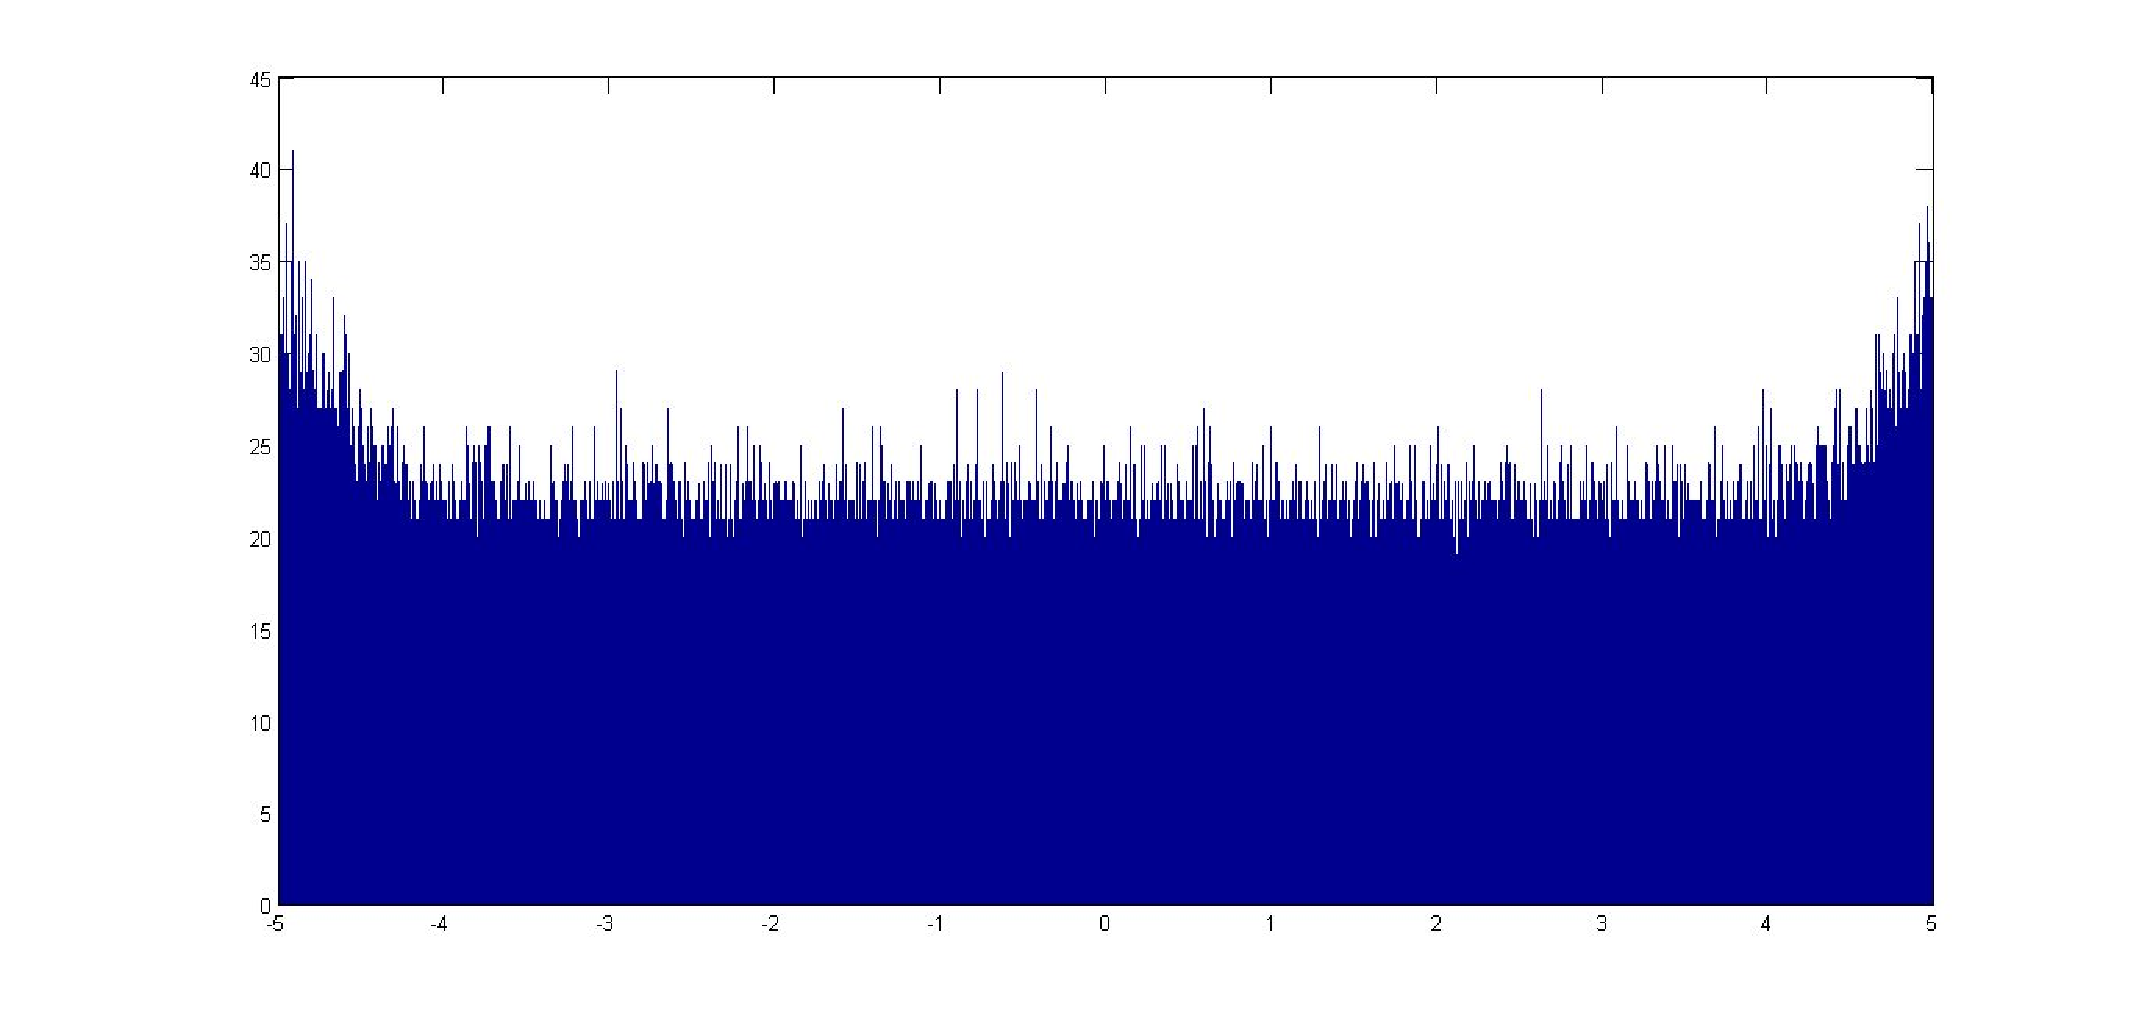
\includegraphics[width=\textwidth]{c_n_20M_1__5_5_2}
\caption{Rozkład normalny}
\end{figure}

\begin{figure}[H]
\centering
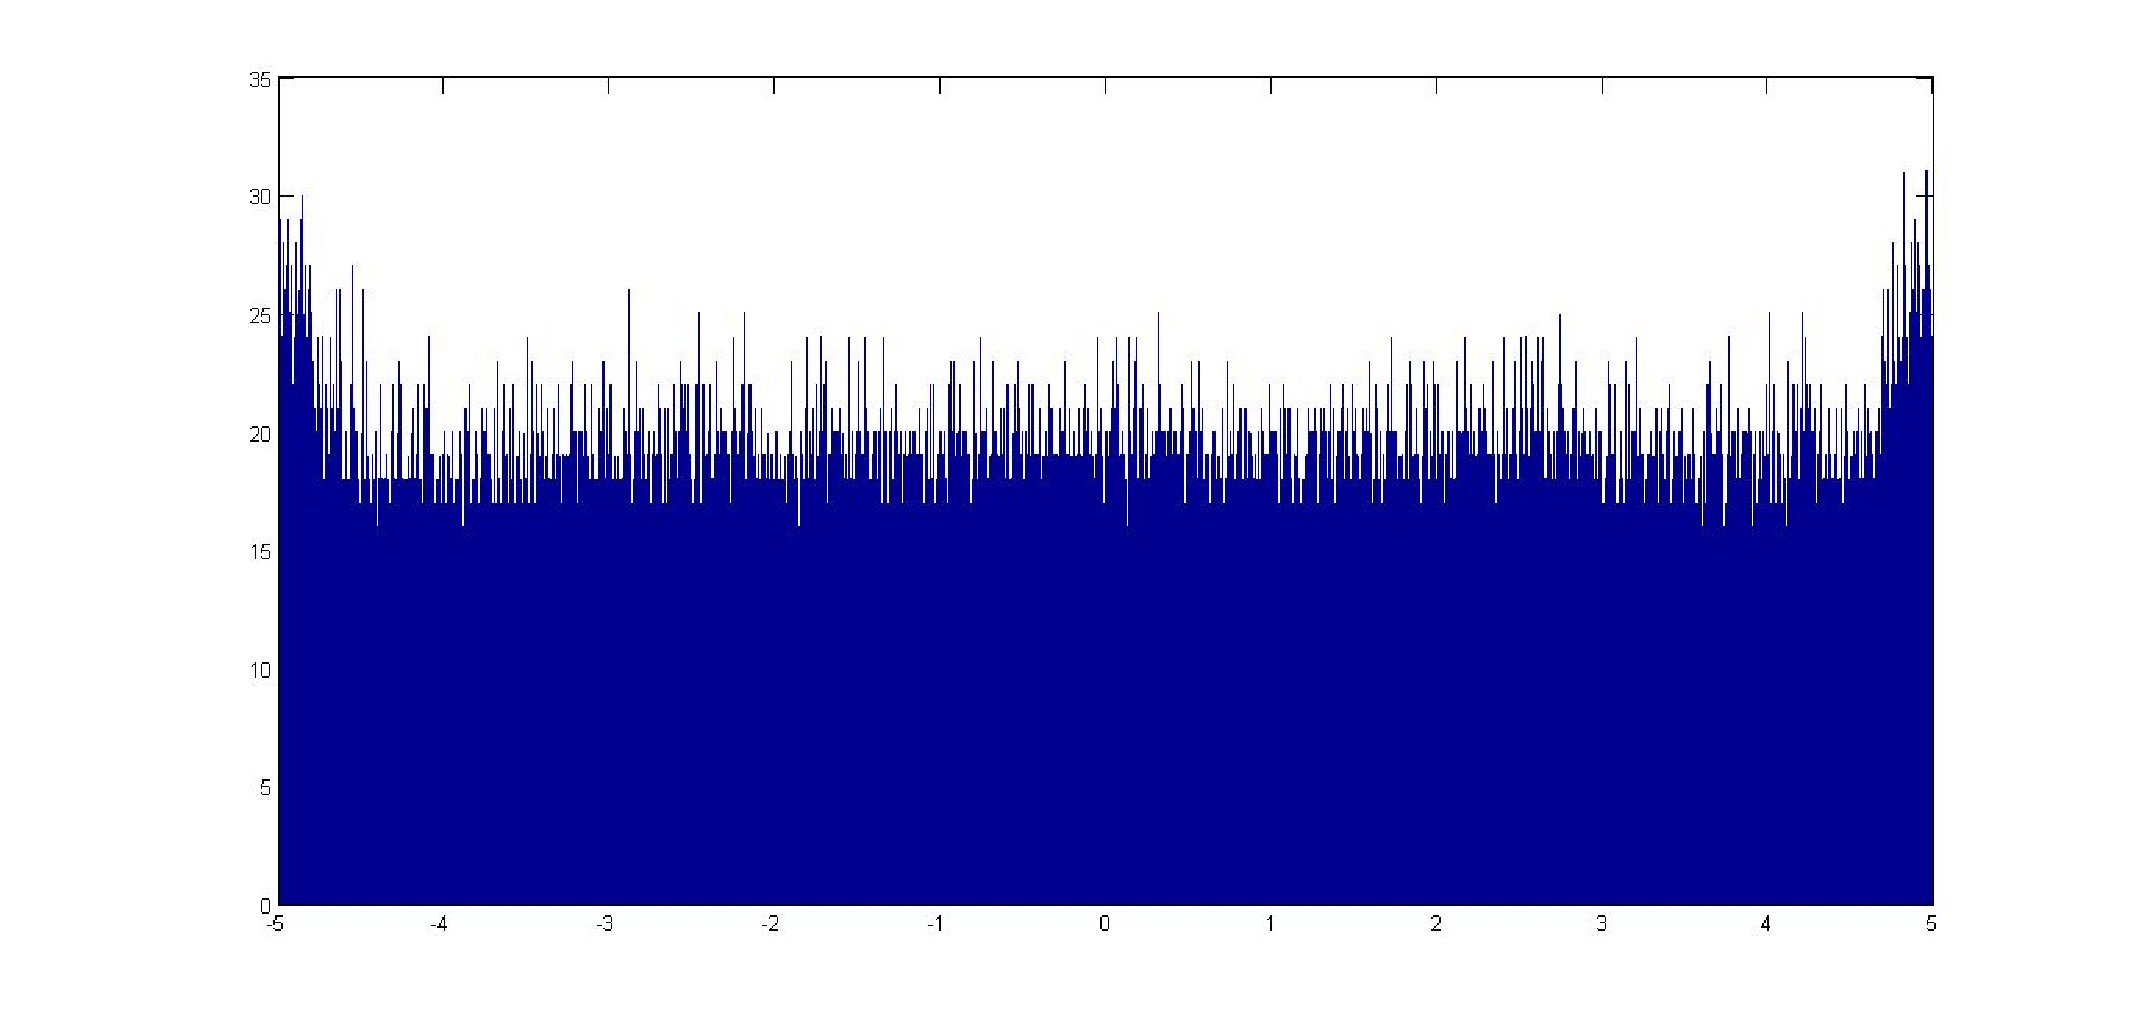
\includegraphics[width=\textwidth]{c_j_2M_1__5_5}
\caption{Rozkład jednostajny}
\end{figure}

\begin{figure}[H]
\centering
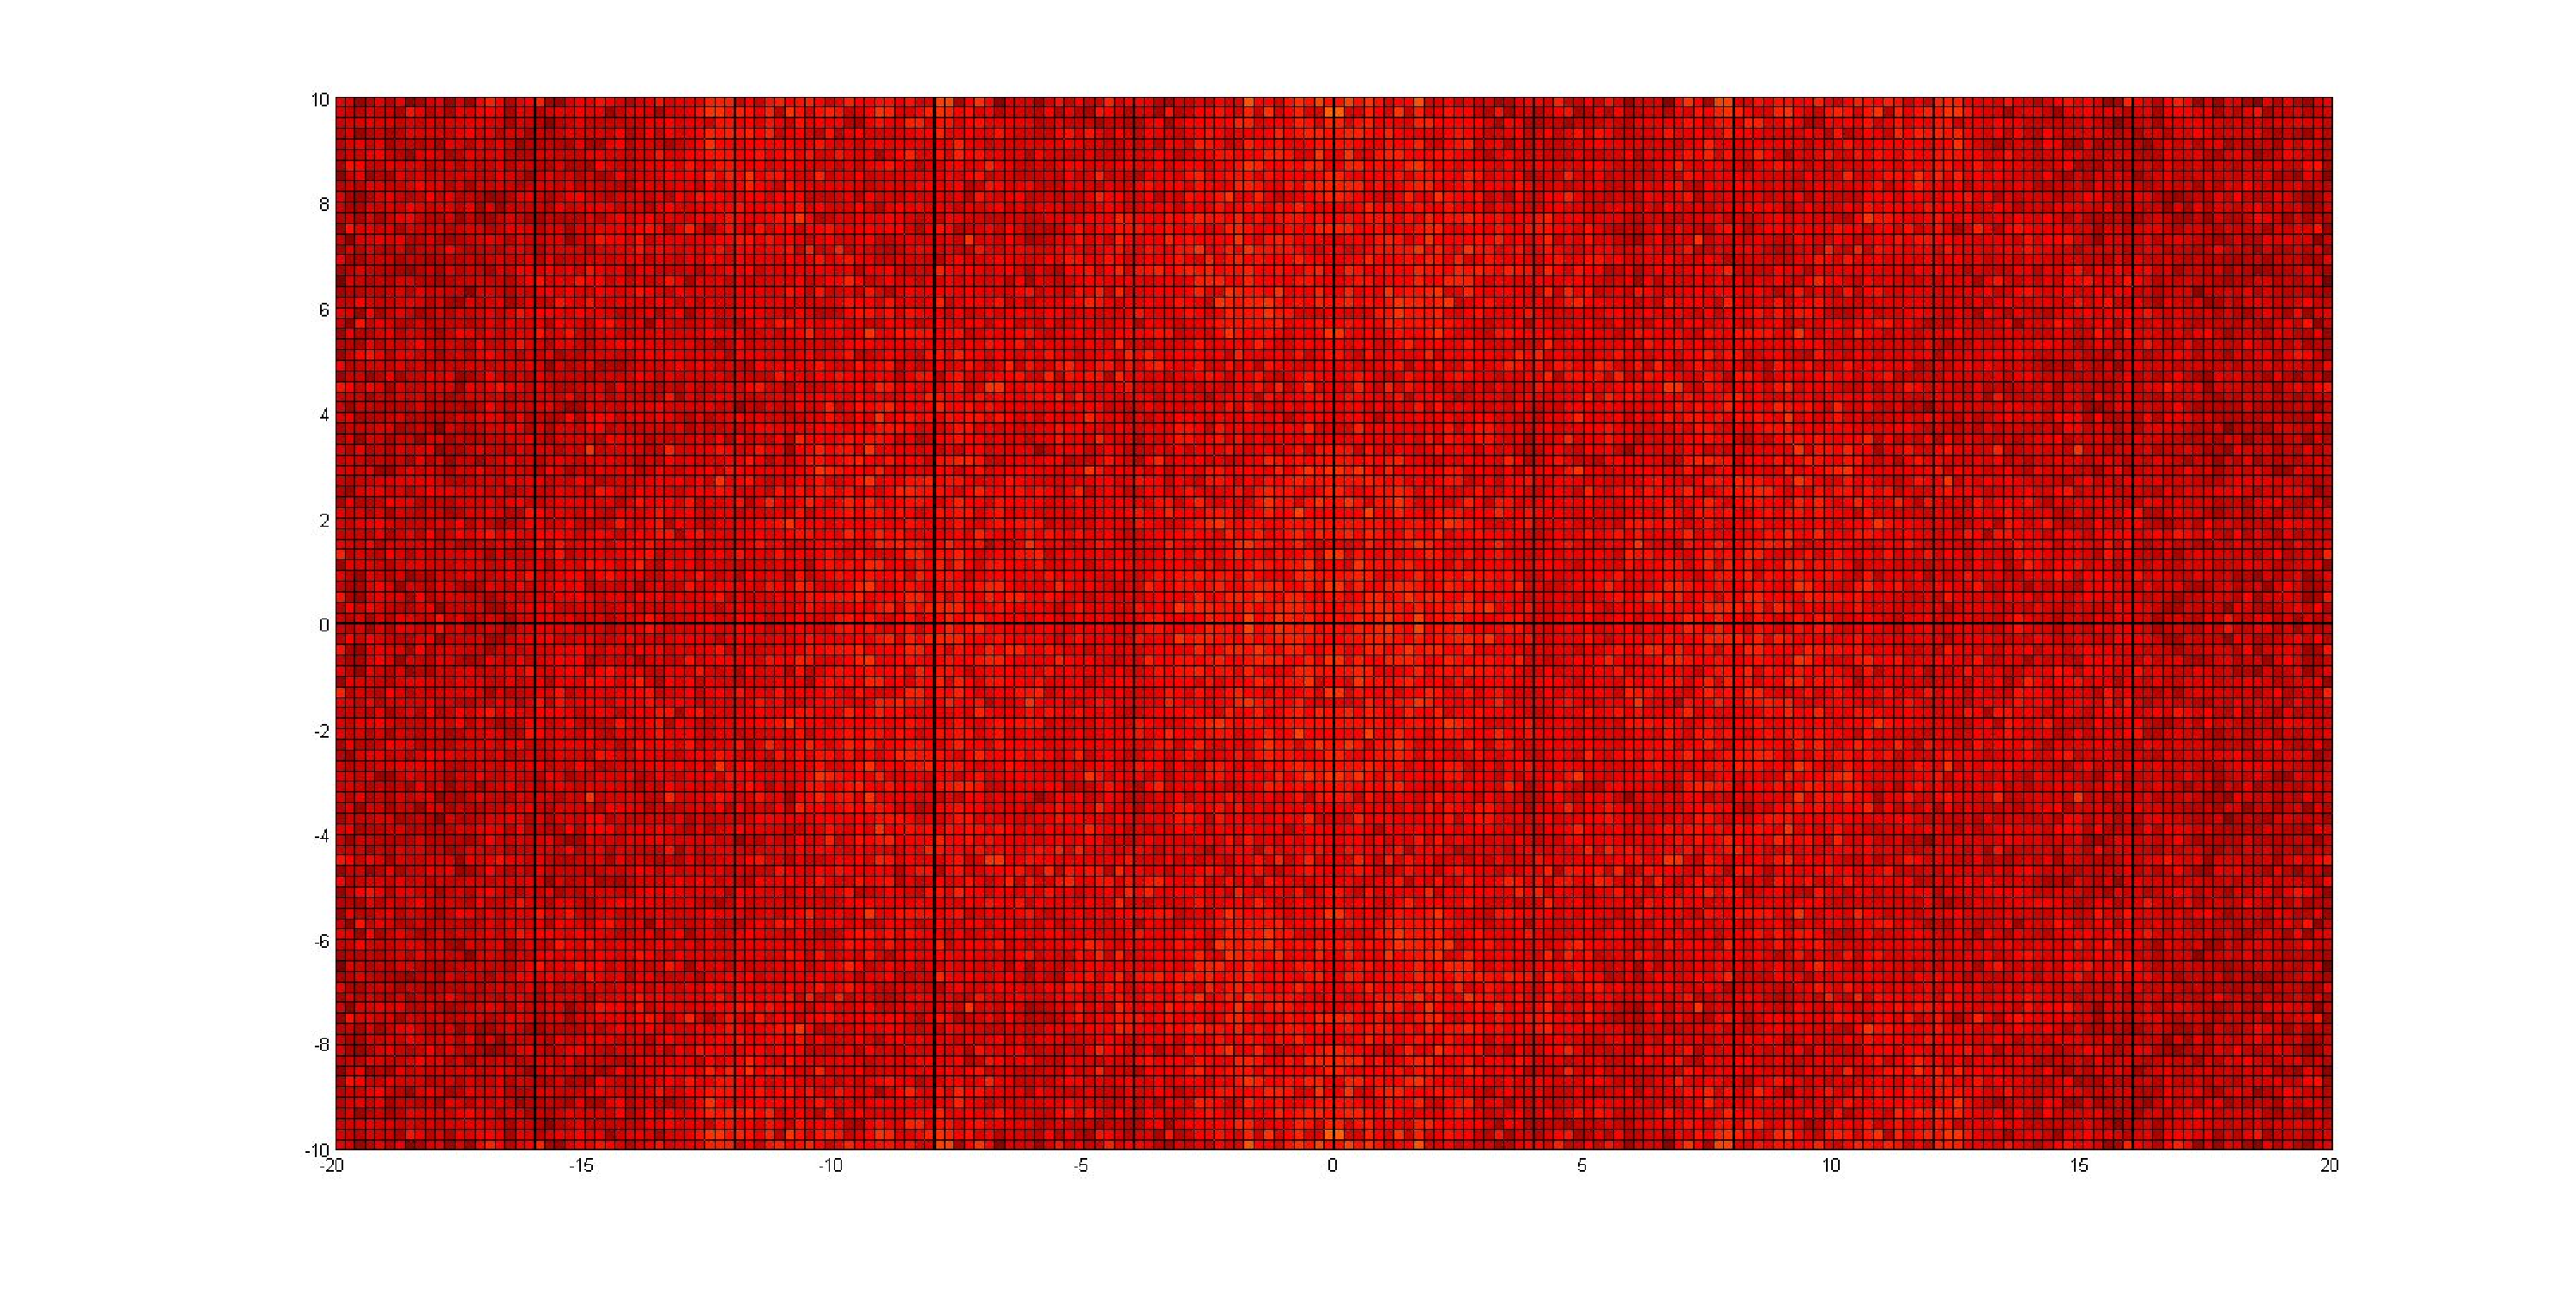
\includegraphics[width=\textwidth]{c_n_10M_2__20_20__10_10_4}
\caption{Rozkład normalny na dwóch wymiarach z kopiowaniem symetrycznym}
\end{figure}

\subsubsection*{Rzutowanie}
Zgodnie z przewidywaniami największe prawdopodobieństwo wystąpienia punktu jest na ograniczeniu, co bardzo dobrze obrazuje rysunek \ref{bladzenie:rzutowanie2d}. Na rysunkach   \ref{bladzenie:rzutowanie1dn} i  \ref{bladzenie:rzutowanie1dj} zakres osi~Y został zmniejszony do odpowiednio $[30000;60000]$ i $[70000;140000]$, aby uwypuklić interesujące efekty. W związku z tym zostały "ucięte" wartości na przedziałach brzegowych. Warto zwrócić uwagę na bardzo niespodziewane zjawisko - wartości histogramów blisko ograniczeń są zdecydowanie mniejsze, niż pozostałe. Oznacza to, że punkty w tych przedziałach występują z mniejszym prawdopodobieństwem, niż pozostałe. Wydawać by się mogło, że powinno być inaczej, ponieważ podczas symulacji punkty często są rzutowane na ograniczenie. Dodatkowo w rozkładzie jednostajnym widać, że istnieją przedziały, w których punkty występują z większym prawdopodobieństwem. Autorom nie udało się formalnie uzasadnić tego zjawiska. Intuicja prowadzi do hipotezy, że punkty, które teoretycznie wypadły bez naprawy zapełniłyby utworzony "dołek", natomiast naprawa sprawia, że cała dalsza symulacja niejako zostaje przesunięta. W ten sposób powstaje "górka" w rozkładzie jednostajnym. Z charakterystyki rozkładu normalnego może brać się fakt, iż owa górka nie występuje w tymże.

\begin{figure}[H]
\centering
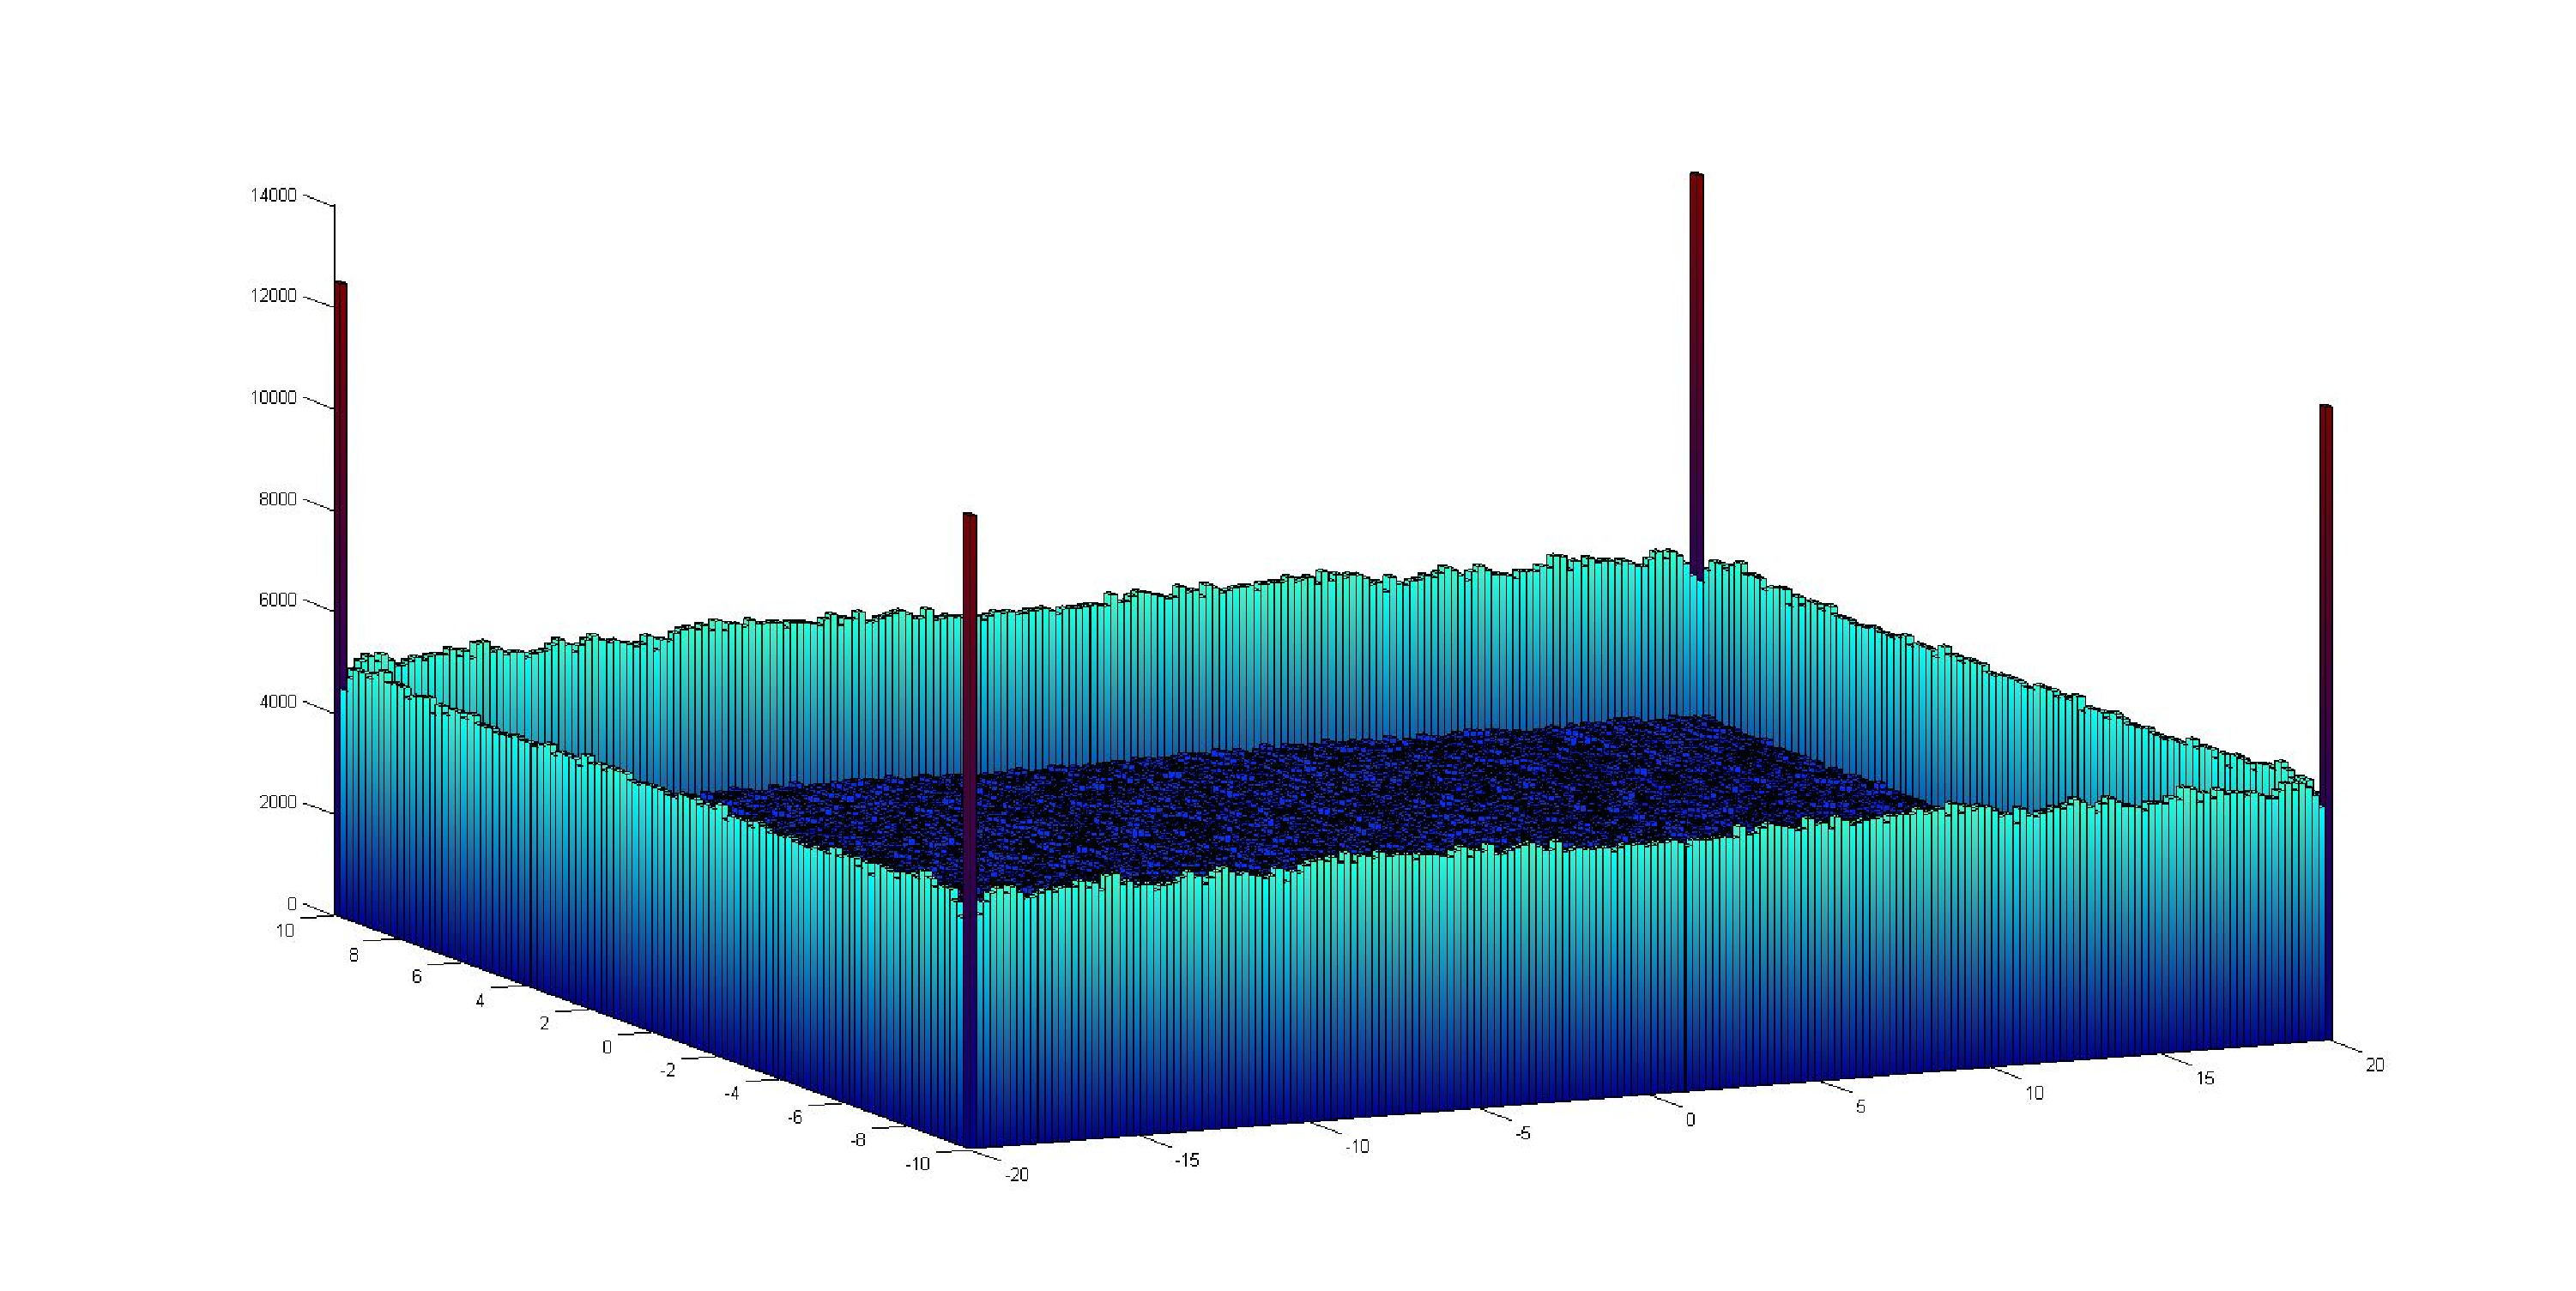
\includegraphics[width=\textwidth]{p_n_10M_2__20_20__10_10_4_2}
\caption{Rozkład normalny na dwóch wymiarach z kopiowaniem symetrycznym}
\label{bladzenie:rzutowanie2d}
\end{figure}

\begin{figure}[H]
\centering
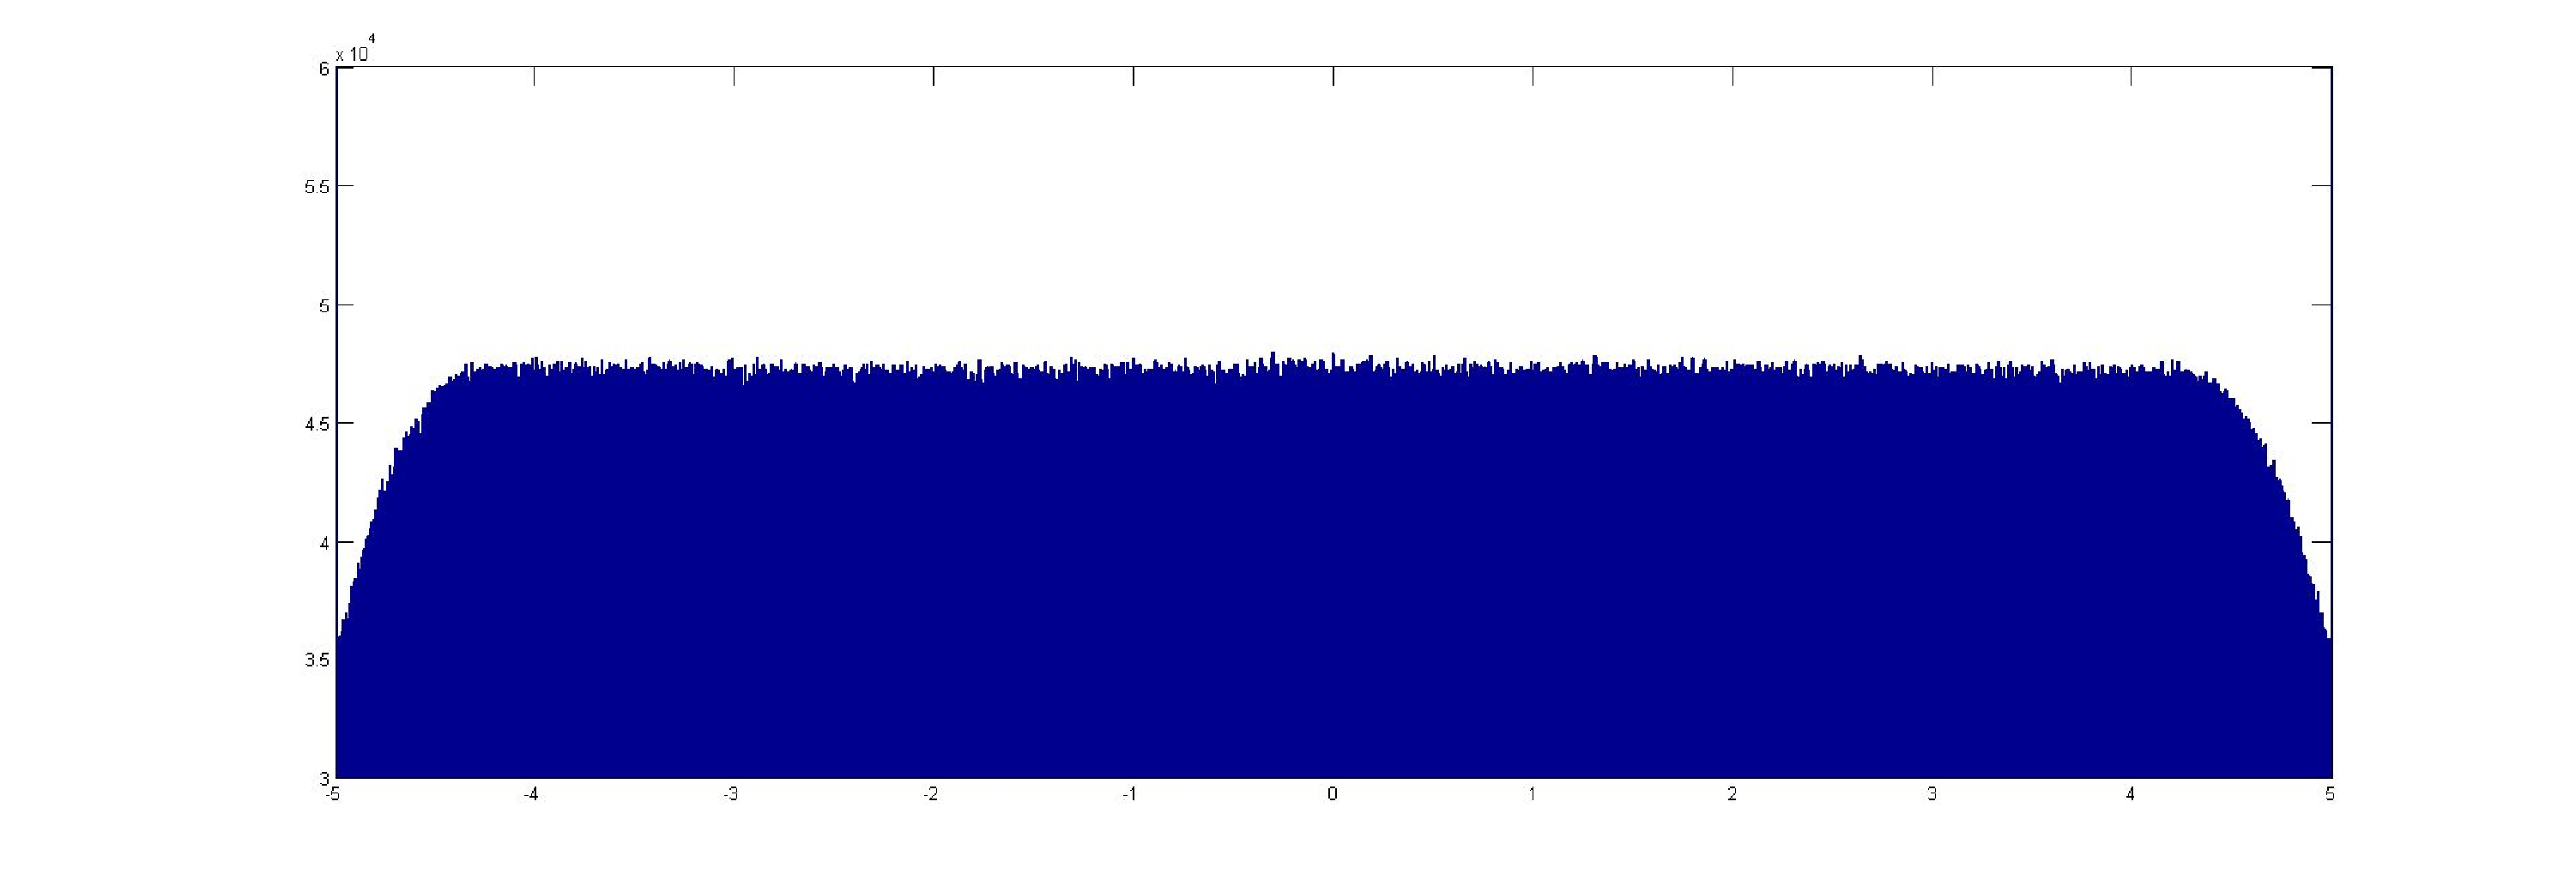
\includegraphics[width=\textwidth]{p_n_50M_1__5_5}
\caption{Rozkład normalny}
\label{bladzenie:rzutowanie1dn}
\end{figure}

\begin{figure}[H]
\centering
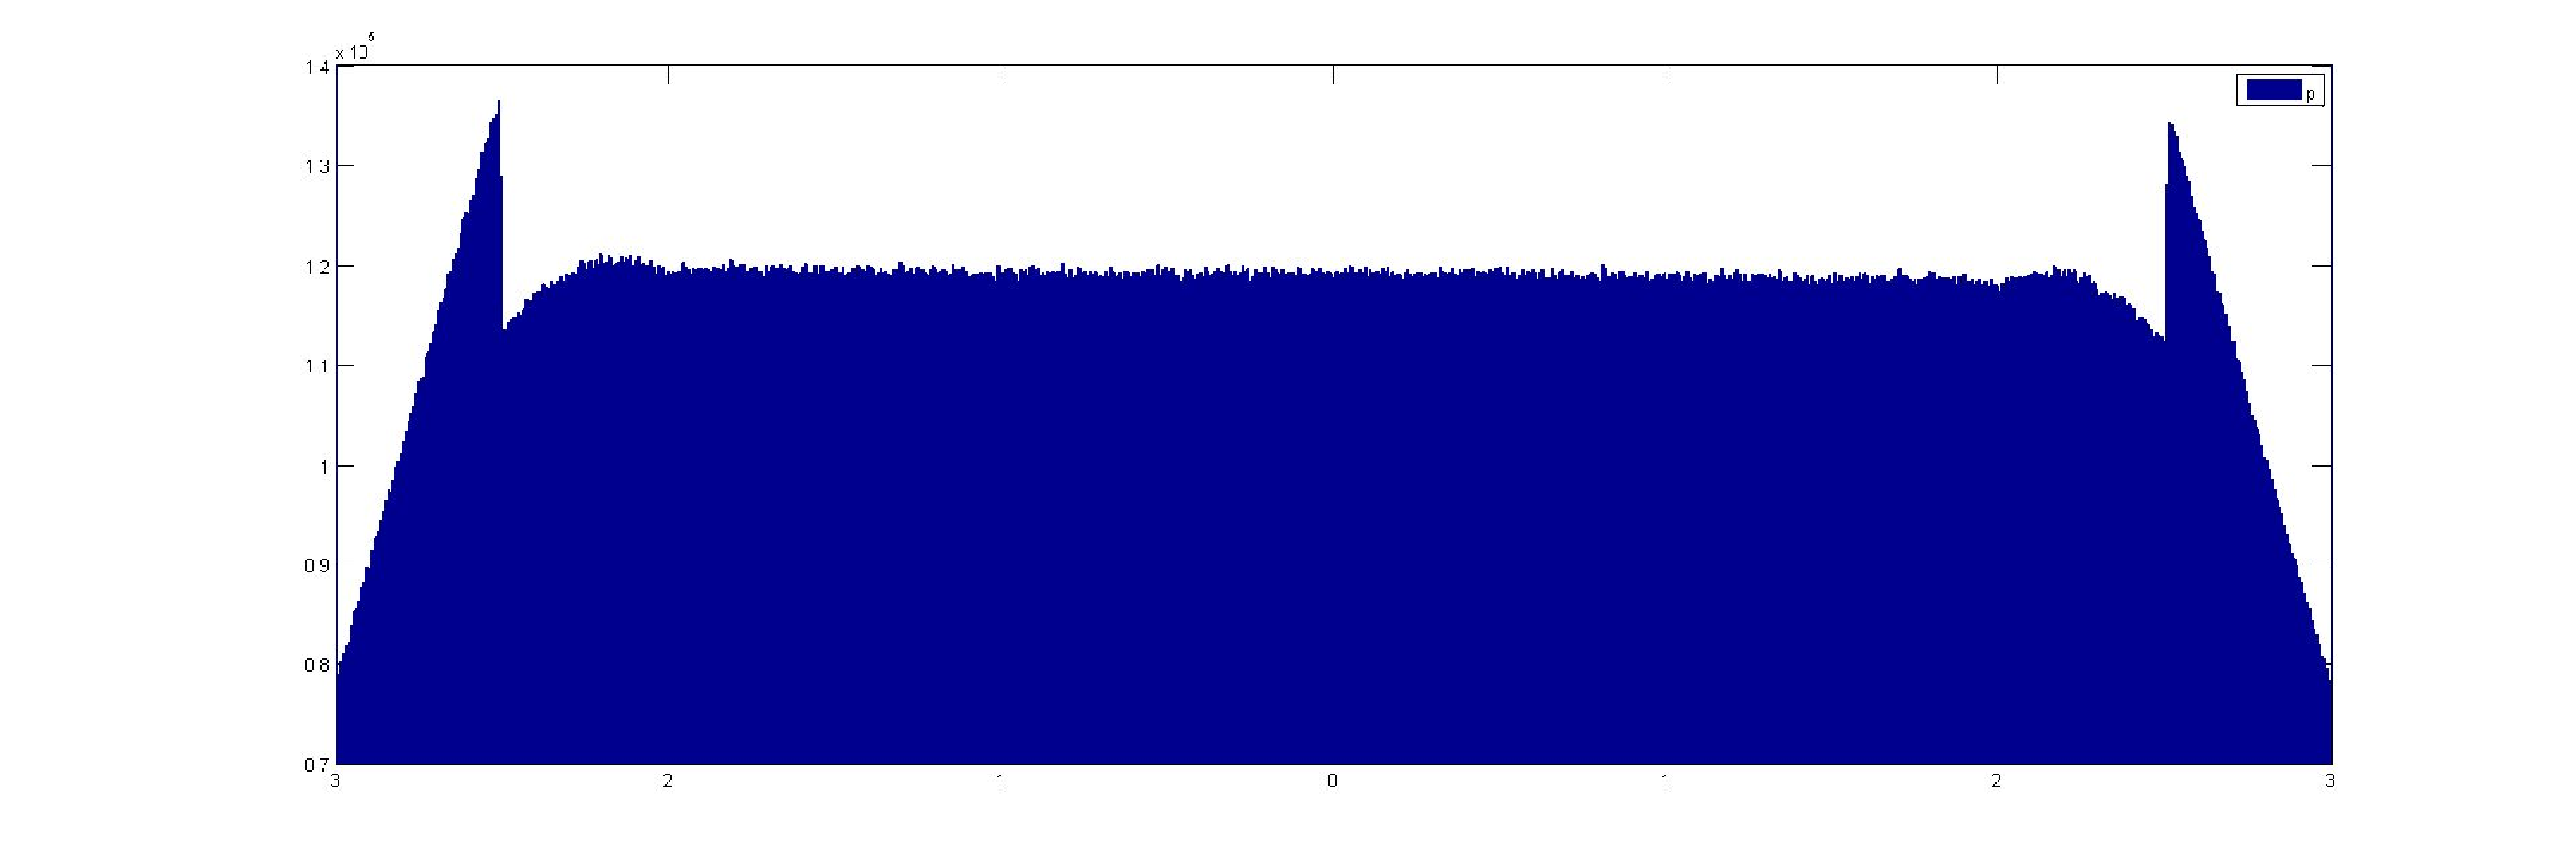
\includegraphics[width=\textwidth]{p_j_100M_1__3_3}
\caption{Rozkład jednostajny}
\label{bladzenie:rzutowanie1dj}
\end{figure}

\subsubsection*{Reinicjalizacja}
Na pierwszy rzut oka wykresy nie ukazują nic nadzwyczajnego, ponieważ łatwo zauważyć pik związany z reinicjalizacją oraz wartości histogramu malejące wraz ze zbliżaniem się do ograniczeń. Autorzy pragną zwrócić uwagę na 2 fakty. Pierwszy, to kształt histogramu. Zarówno dla rozkładu jednostajnego i normalnego w jednym wymiarze jest on stożkowy. Łuk widać tylko blisko punktu środkowego, w pozostałej części spadek jest liniowy. Brakuje charakterystycznego, gaussowskiego przegięcia. Sytuacja jest ciekawsza, gdy występuje więcej wymiarów. Widać wówczas przegięcie. Dokładniejsze badania pokazały, że przegięcie nie występuje tylko na jednym wymiarze. Tym, który jest relatywnie najkrótszy. Celowo jest użyte słowo relatywnie, ponieważ z perspektywy błądzenia przypadkolwego i rozkładu normalnego trzeba brać pod uwagę parametr $\sigma$. Wymiary o małym $\sigma$ będą relatywnie dłuższe od tych z dużym $\sigma$, ponieważ błądzenie będzie wykonywało mniejsze kroki.\\
Na rysunku \ref{bladzenie:probkowanie1dj} można dostrzec też dwa uskoki, które związane są z pikiem w punkcie~$0$ oraz charakterystyką rozkładu.

\begin{figure}[H]
\centering
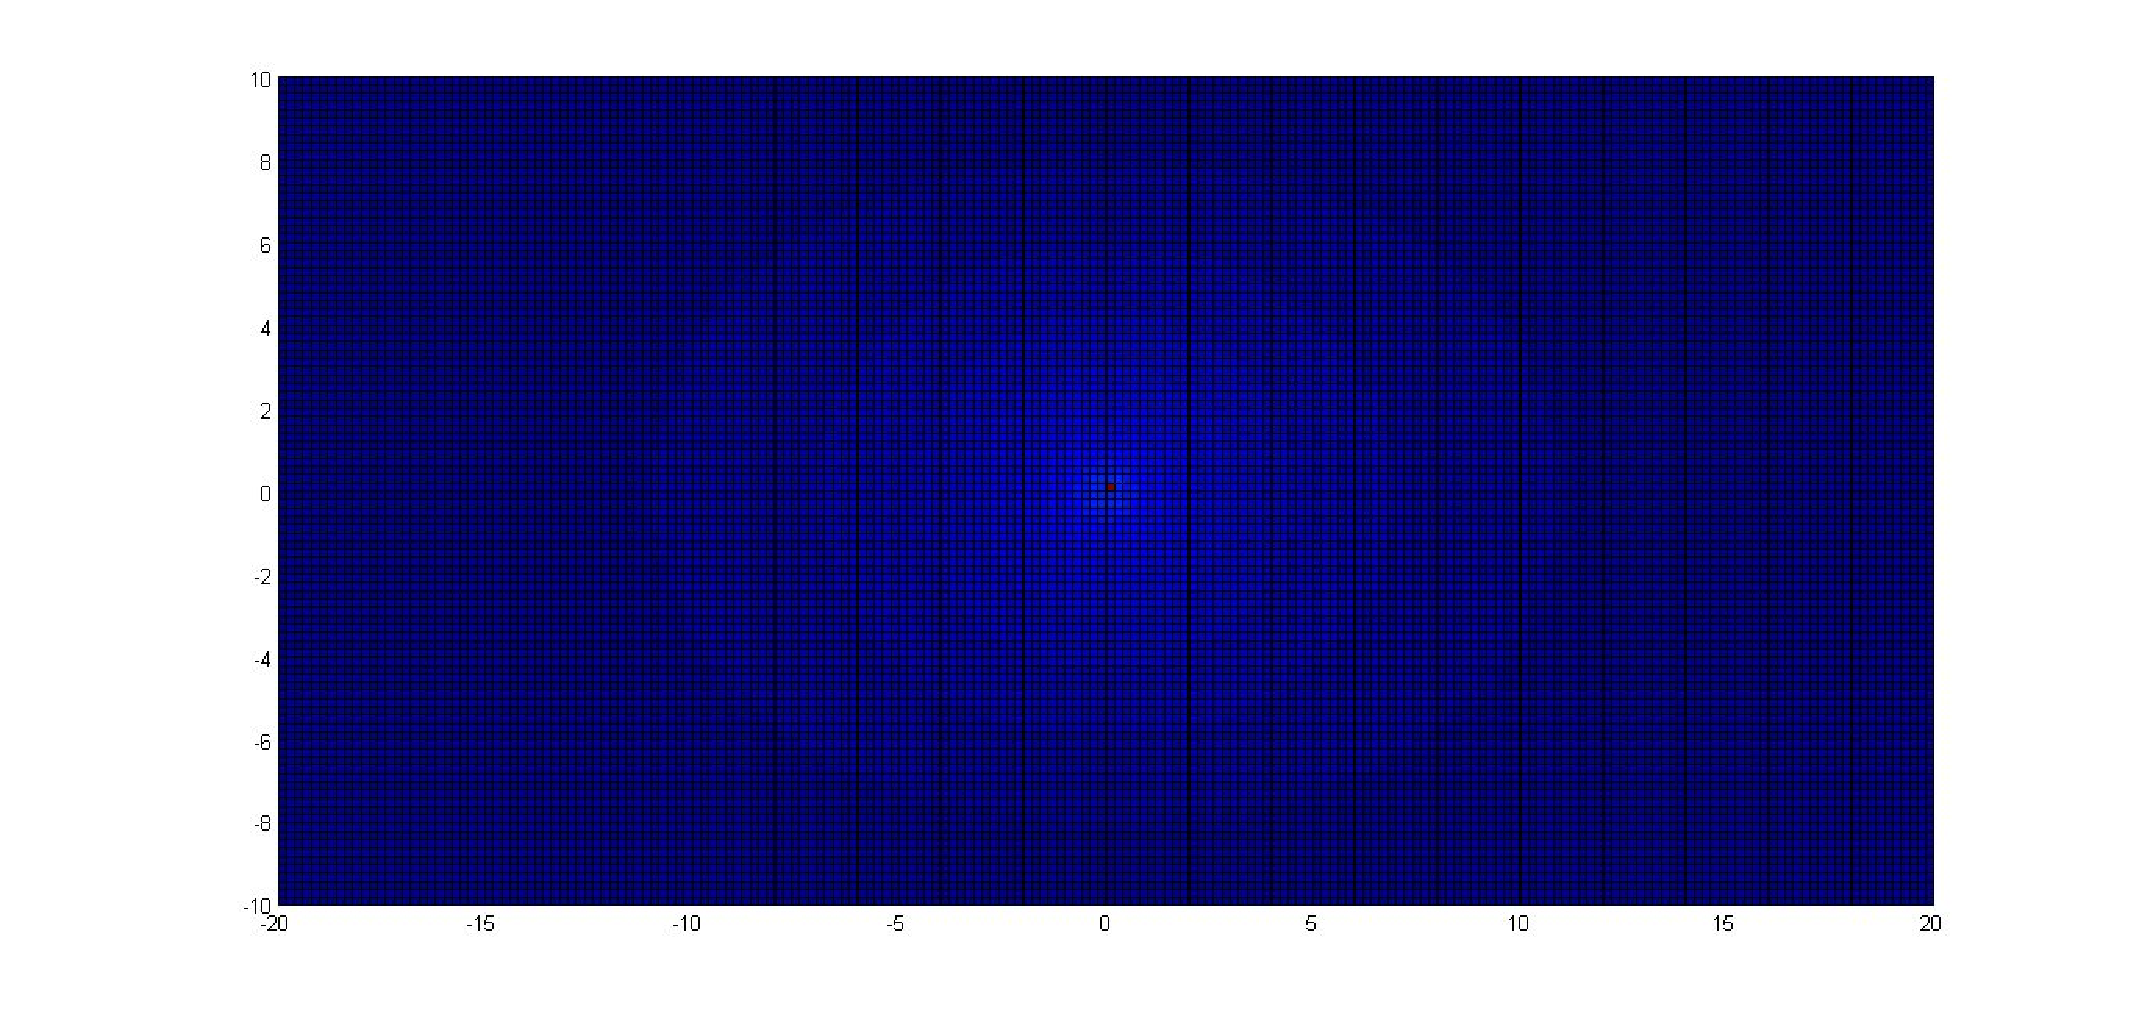
\includegraphics[width=\textwidth]{ri_n_10M_2__20_20__10_10_4}
\caption{Rozkład normalny na dwóch wymiarach z kopiowaniem symetrycznym}
\end{figure}

\begin{figure}[H]
\centering
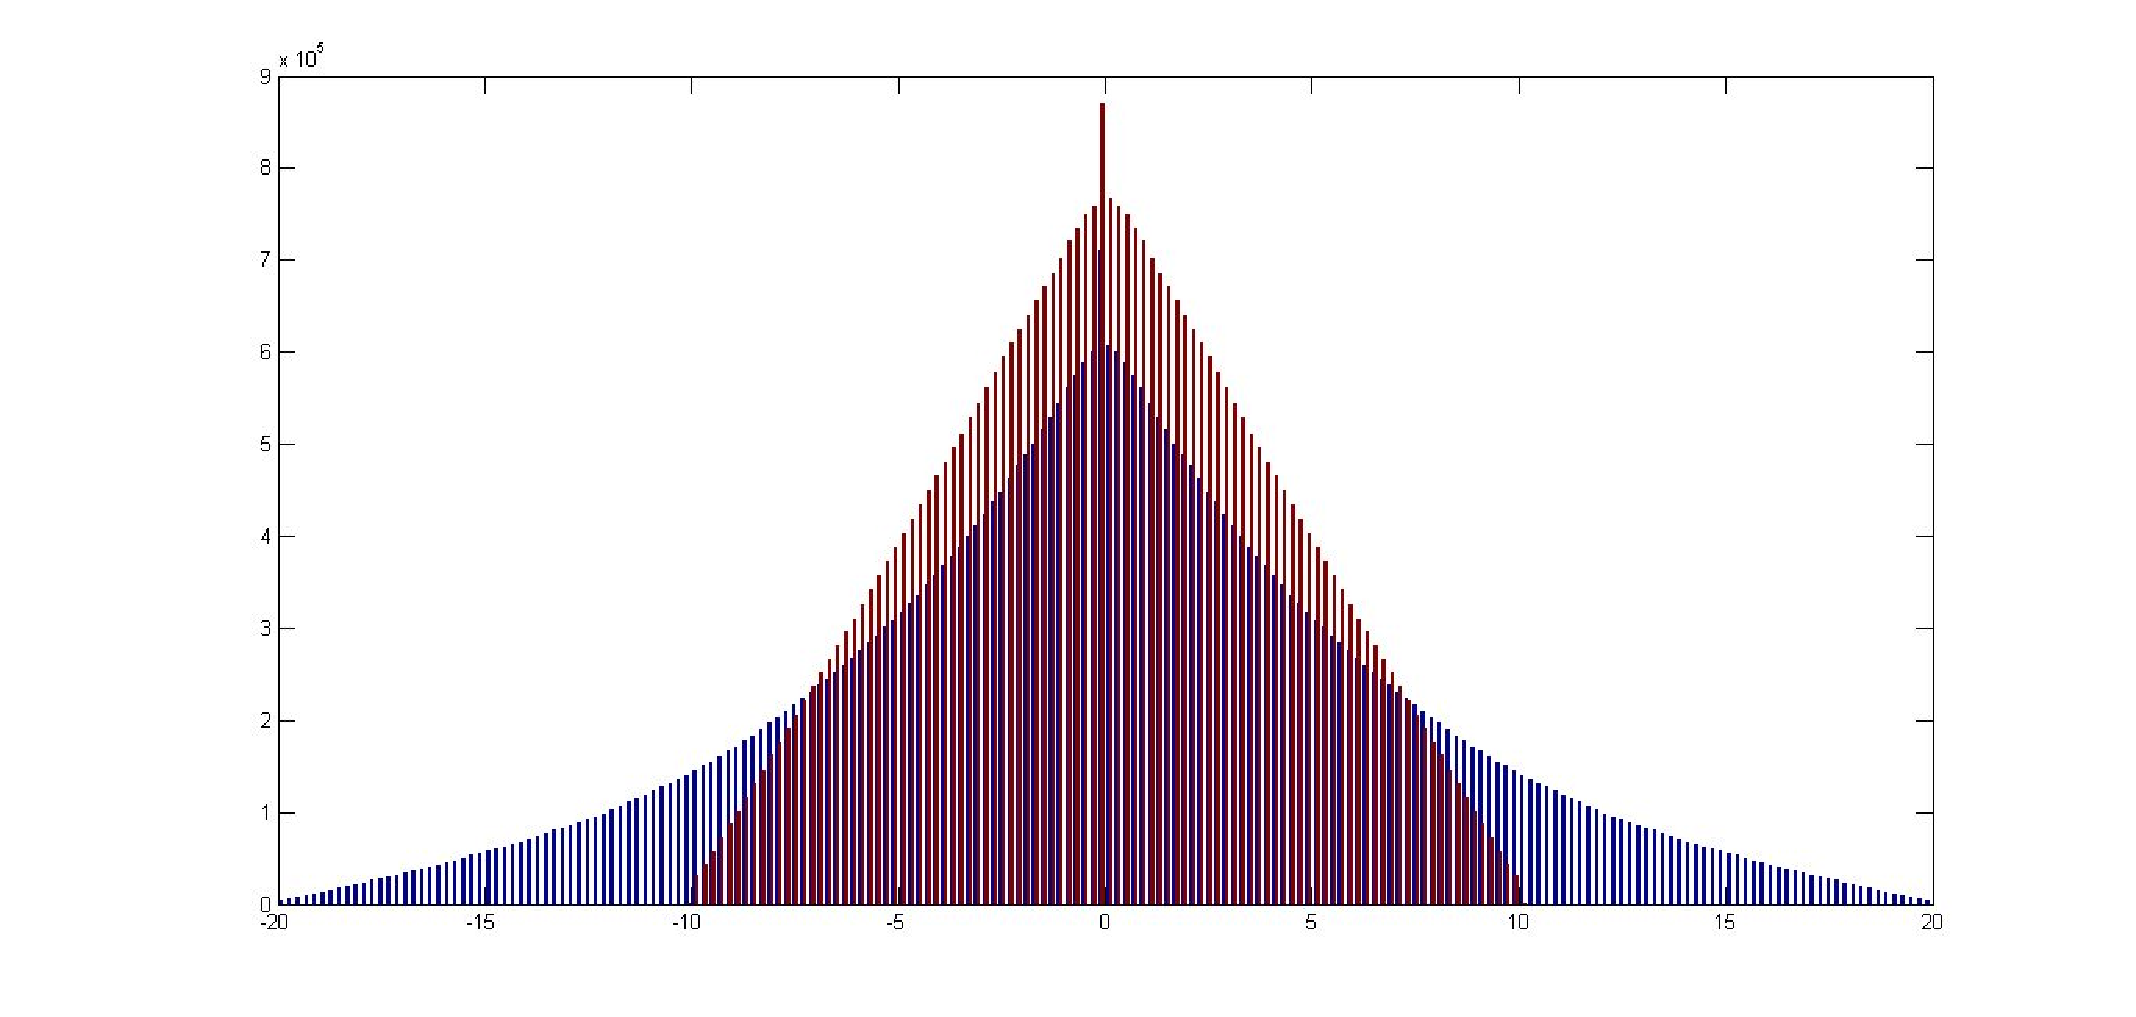
\includegraphics[width=\textwidth]{ri_n_10M_2__20_20__10_10_4_1D}
\caption{Rozkład normalny na dwóch wymiarach z kopiowaniem symetrycznym; oddzielne histogramy dla obu wymiarów}
\end{figure}

\begin{figure}[H]
\centering
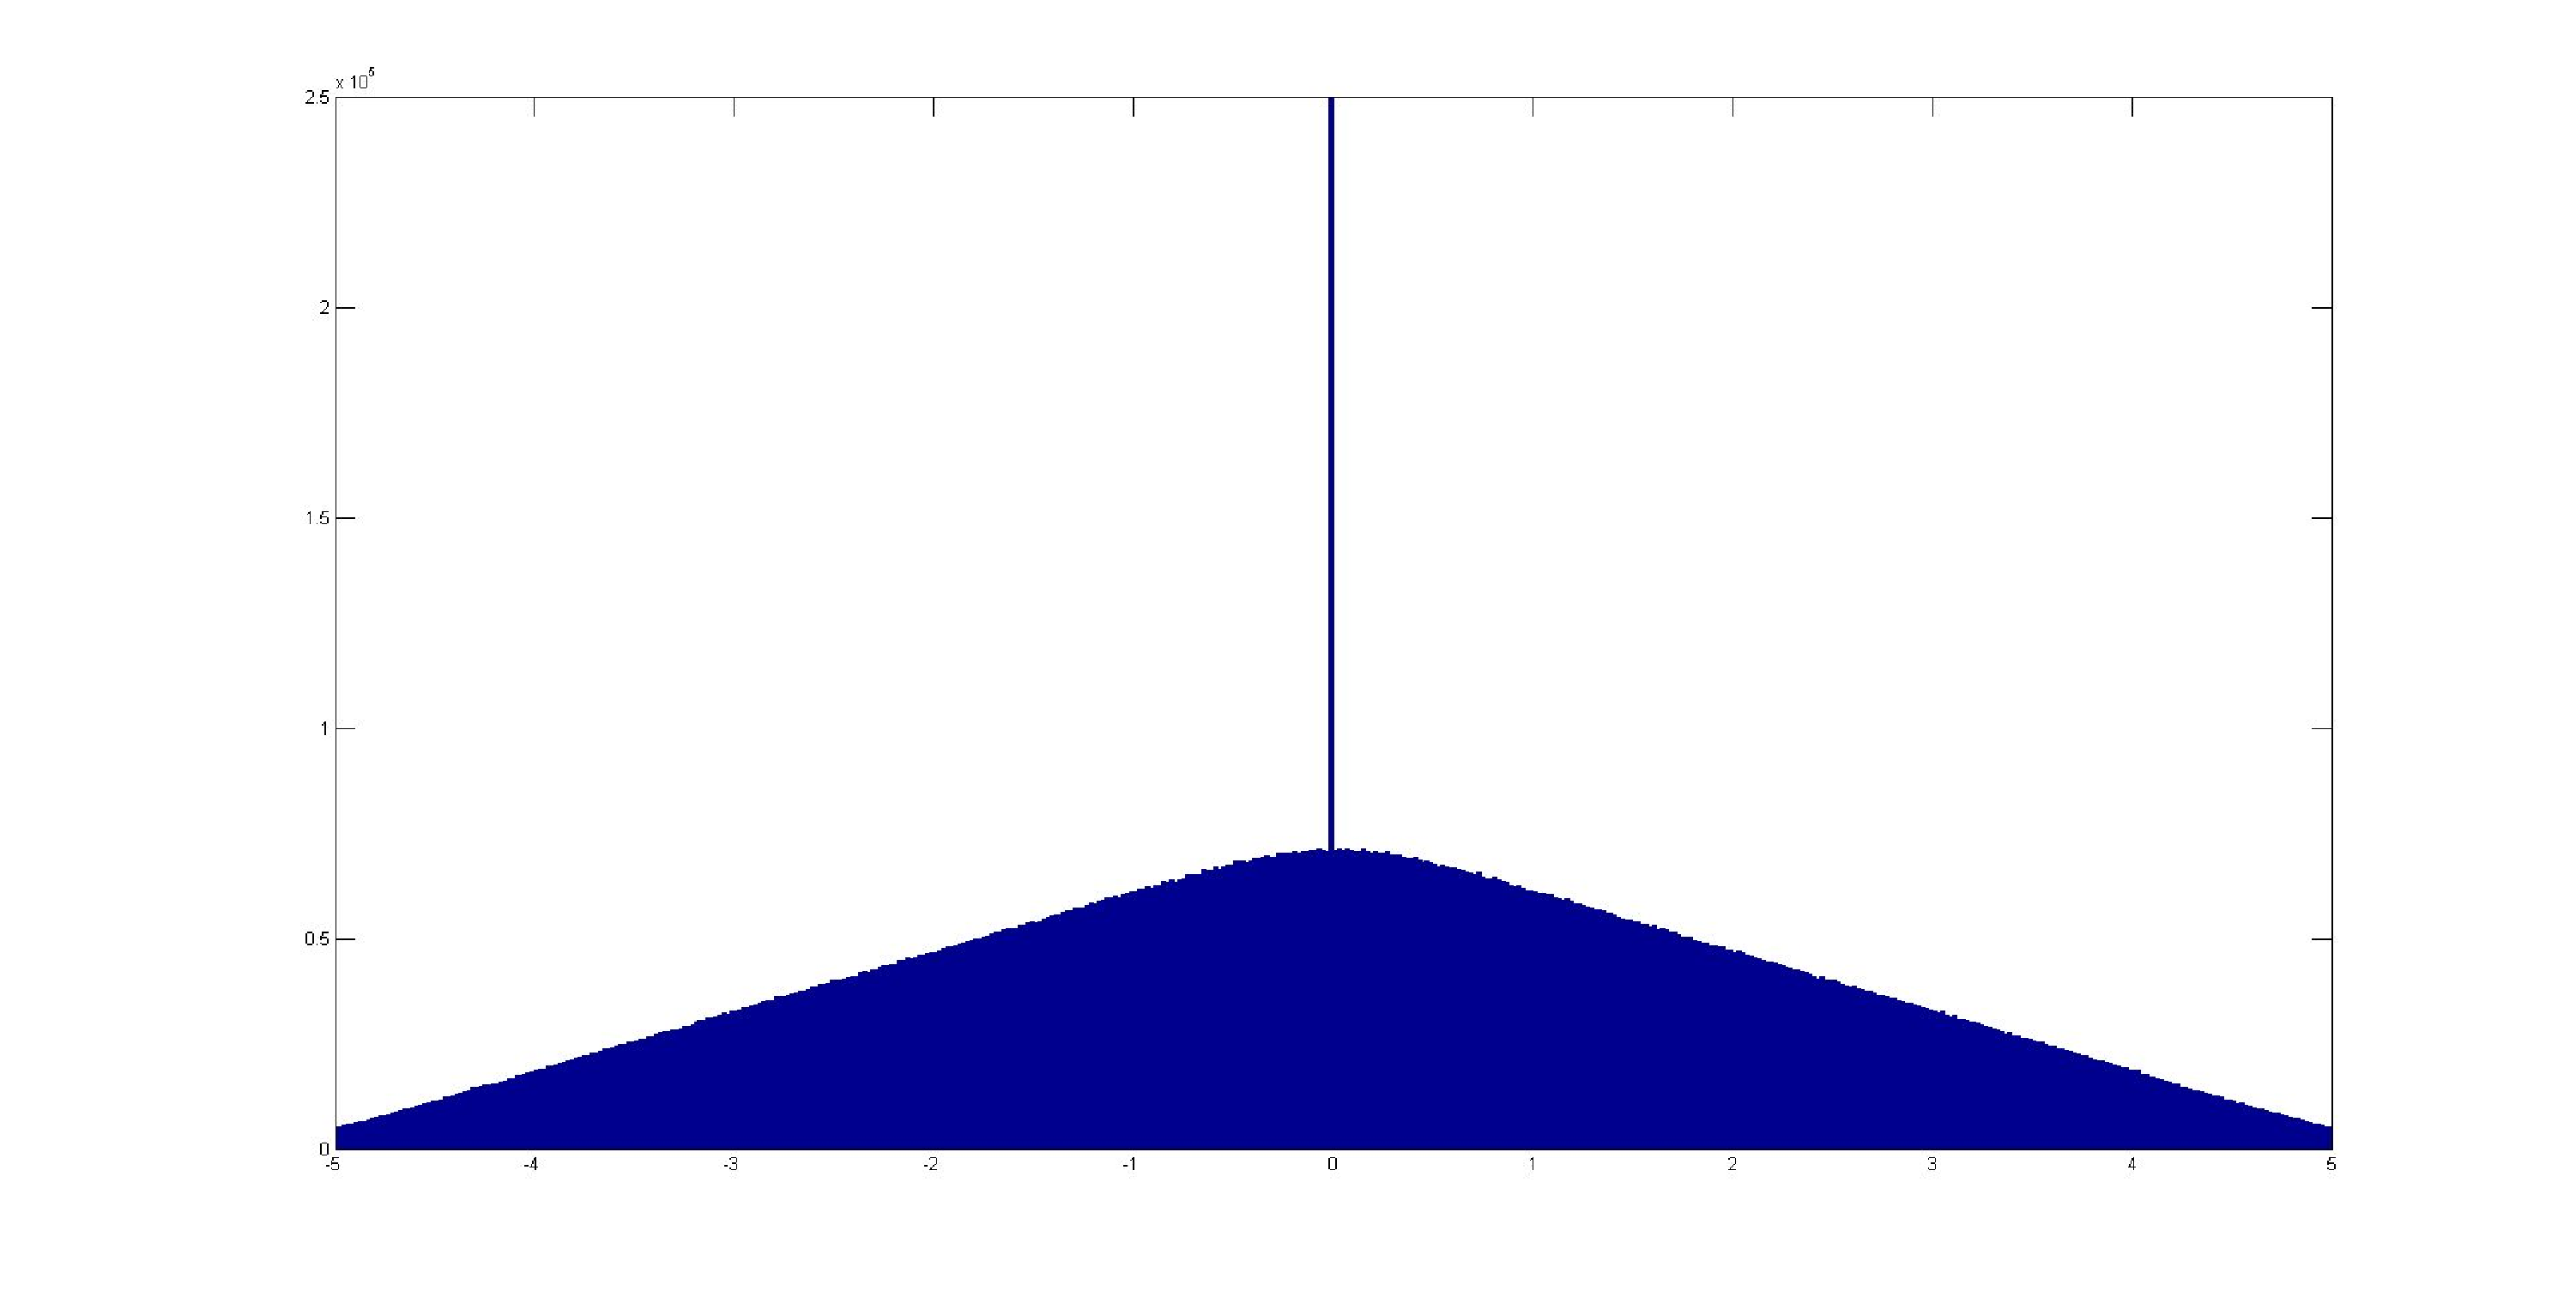
\includegraphics[width=\textwidth]{ri_n_20M_1__5_5}
\caption{Rozkład normalny}
\end{figure}

\begin{figure}[H]
\centering
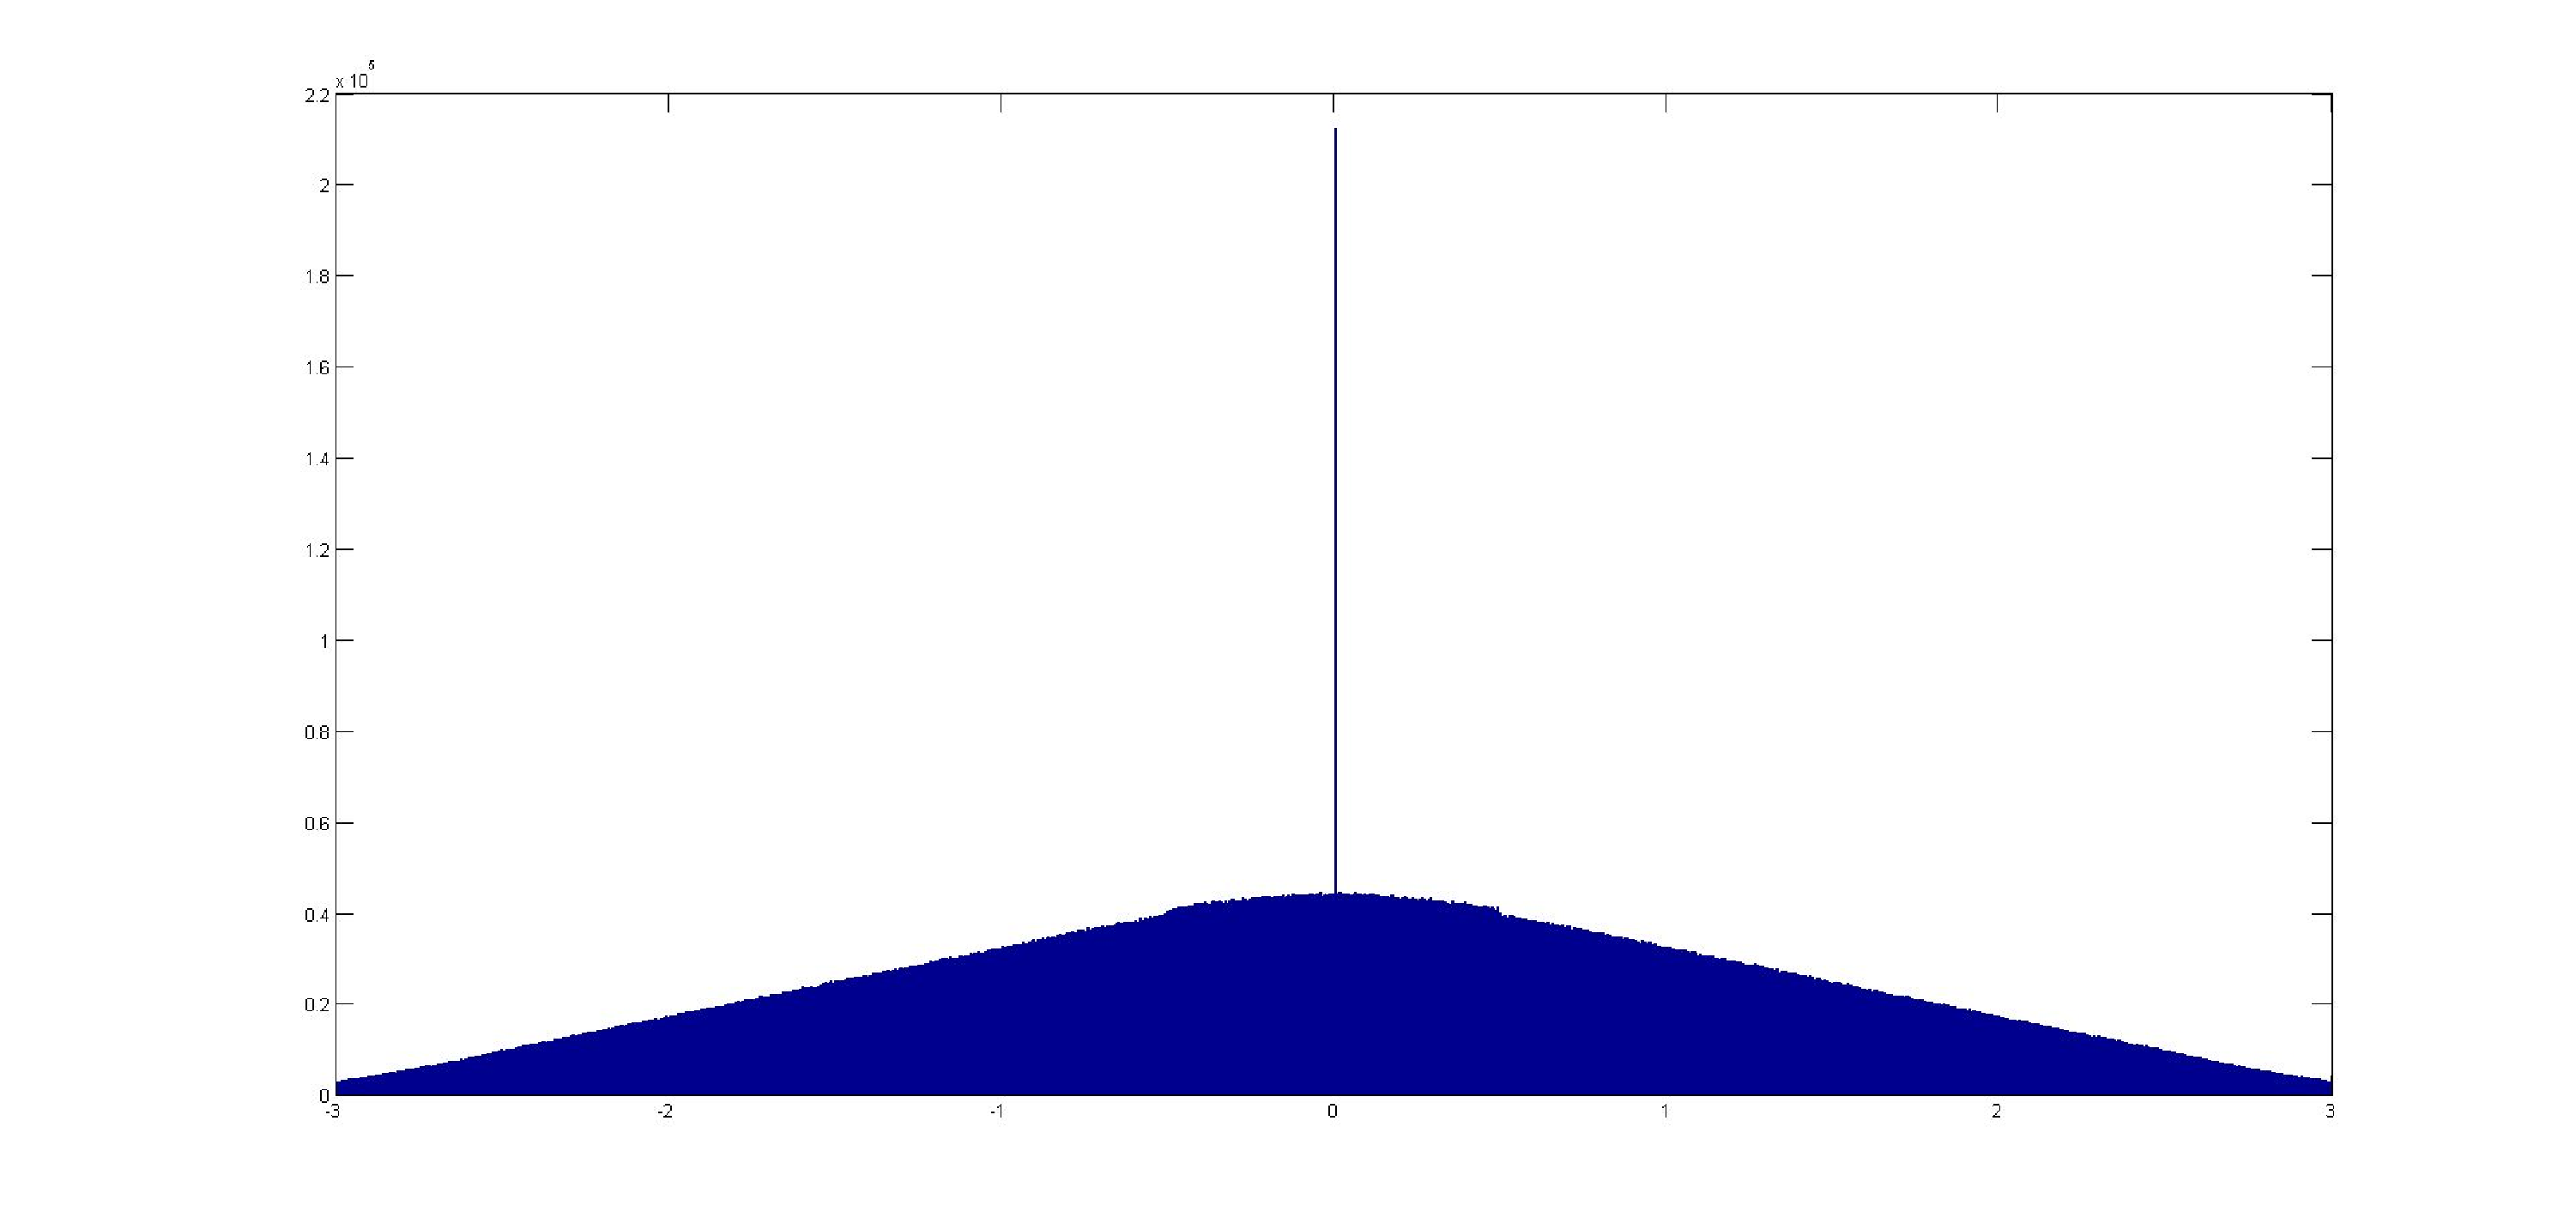
\includegraphics[width=\textwidth]{ri_j_20M_1__3_3}
\caption{Rozkład jednostajny}
\end{figure}

\subsubsection*{Próbkowanie}
Ten rozkład charakteryzuje się spadkiem wartości prawdopodobieństwa wraz z zbliżaniem się do ograniczenia. Punky, które wypadłyby poza ograniczenia oraz ich potomkowie są przesuwane w kierunku środka przedziału.

\begin{figure}[H]
\centering
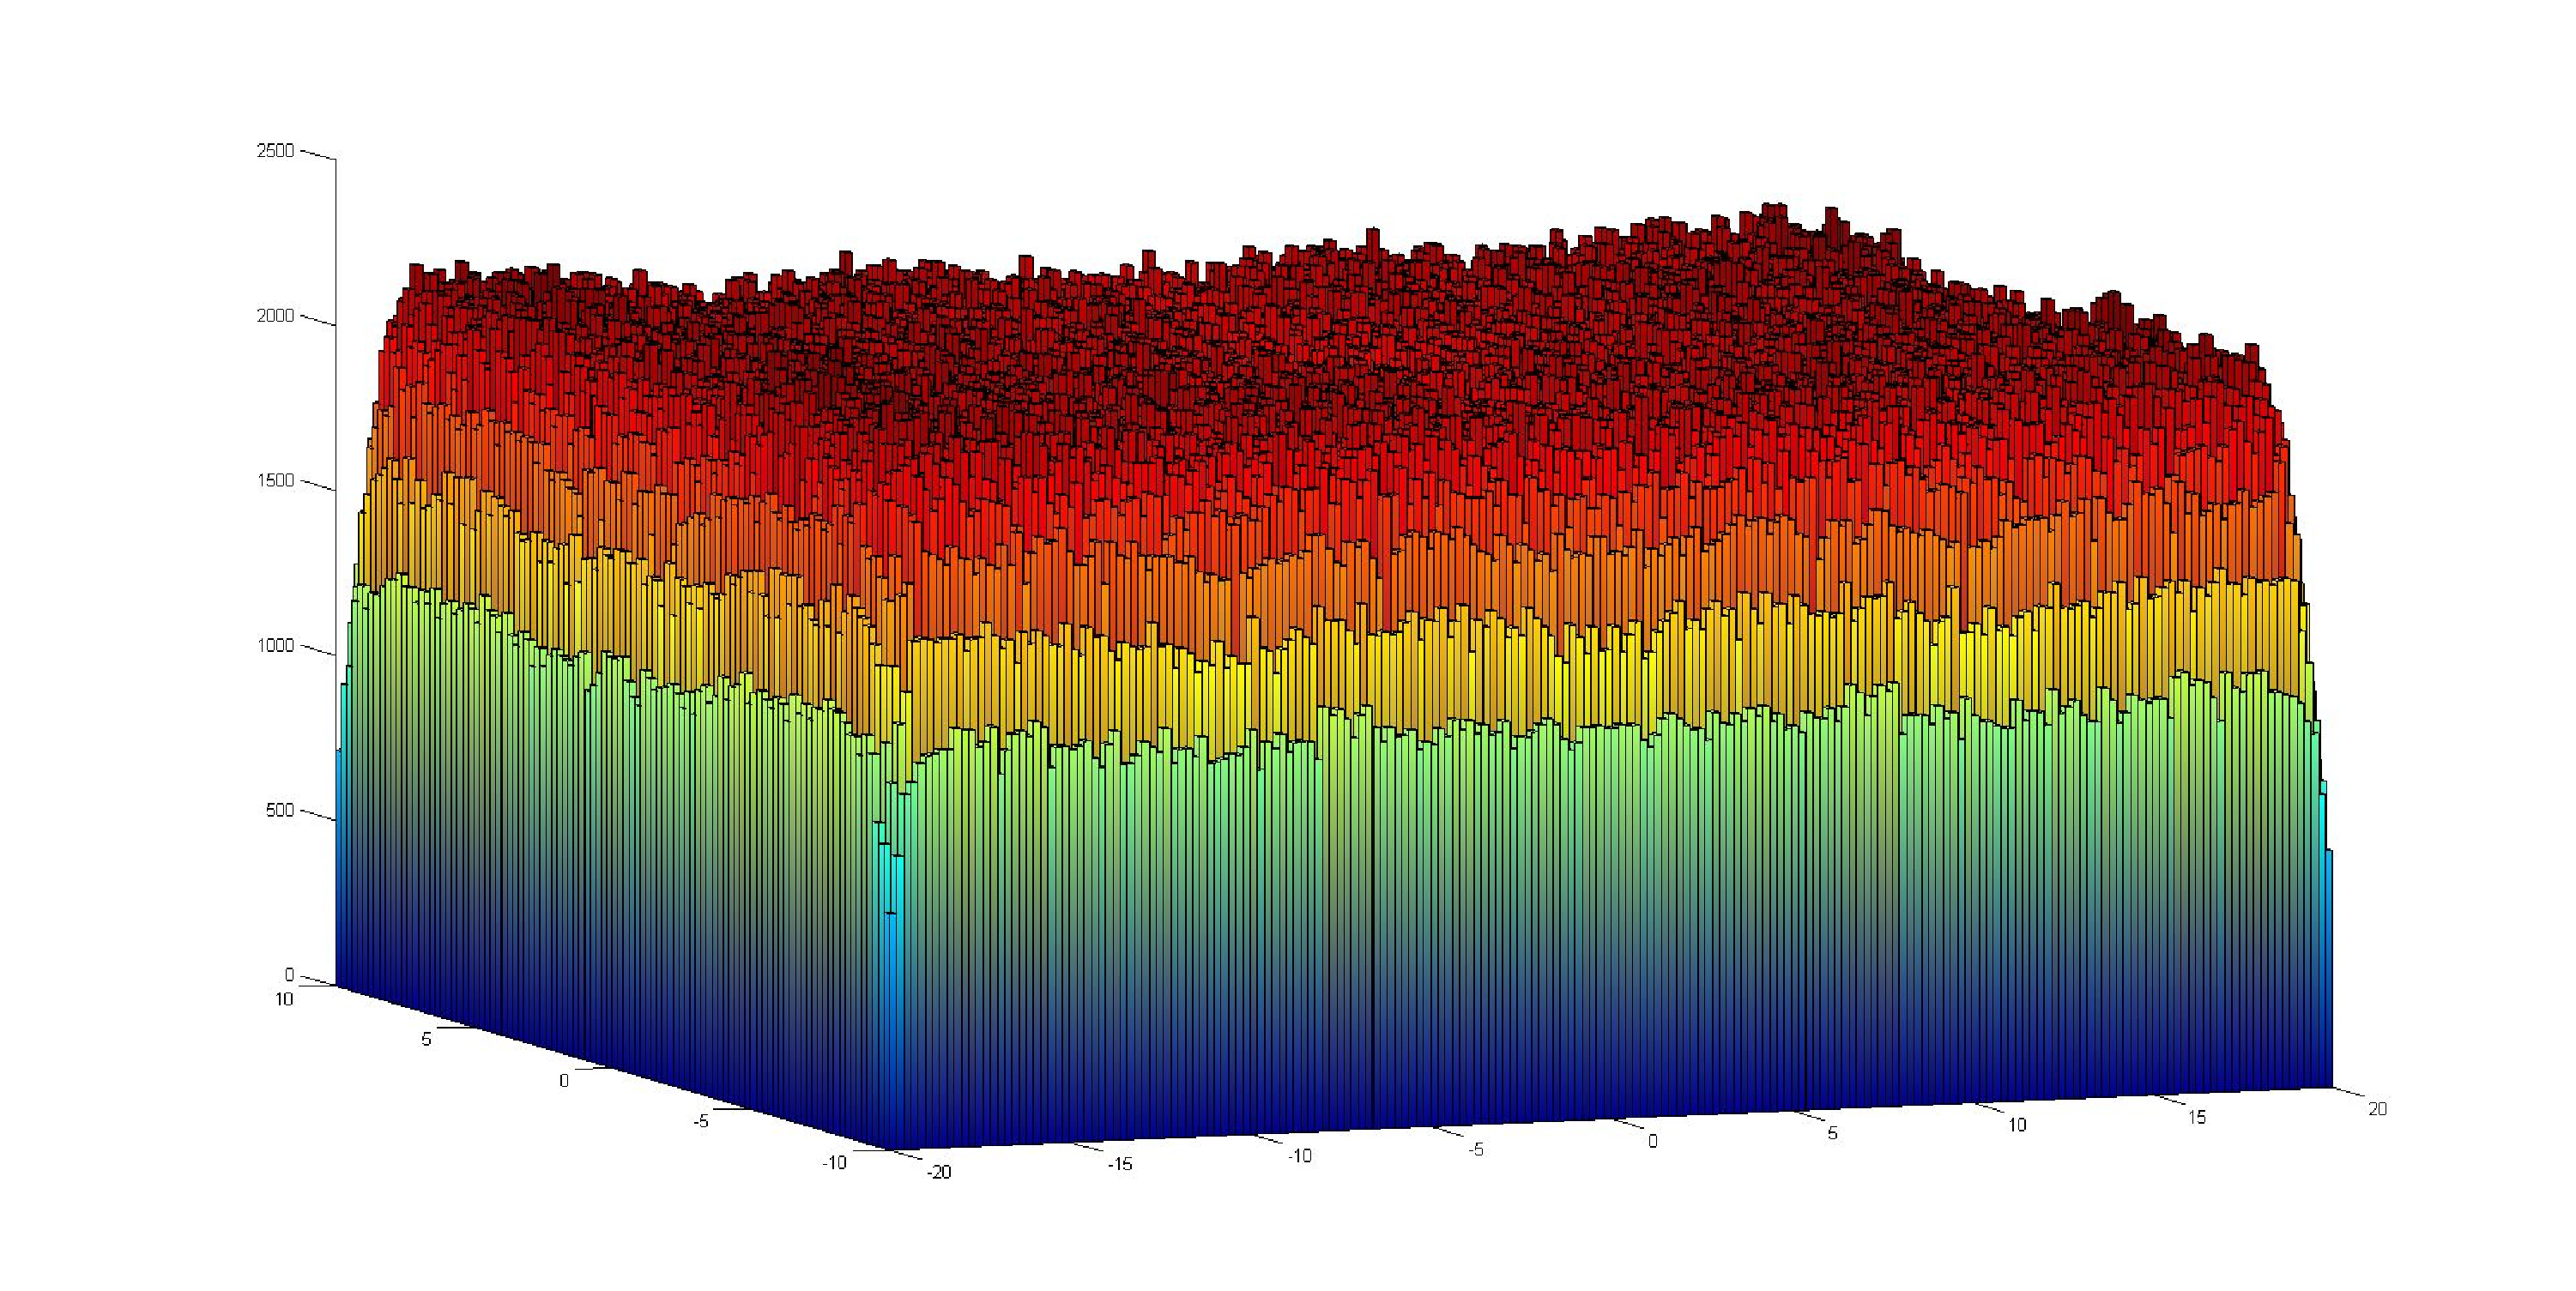
\includegraphics[width=\textwidth]{s_n_10M_2__20_20__10_10_4_2}
\caption{Rozkład normalny na dwóch wymiarach z kopiowaniem symetrycznym}
\end{figure}

\begin{figure}[H]
\centering
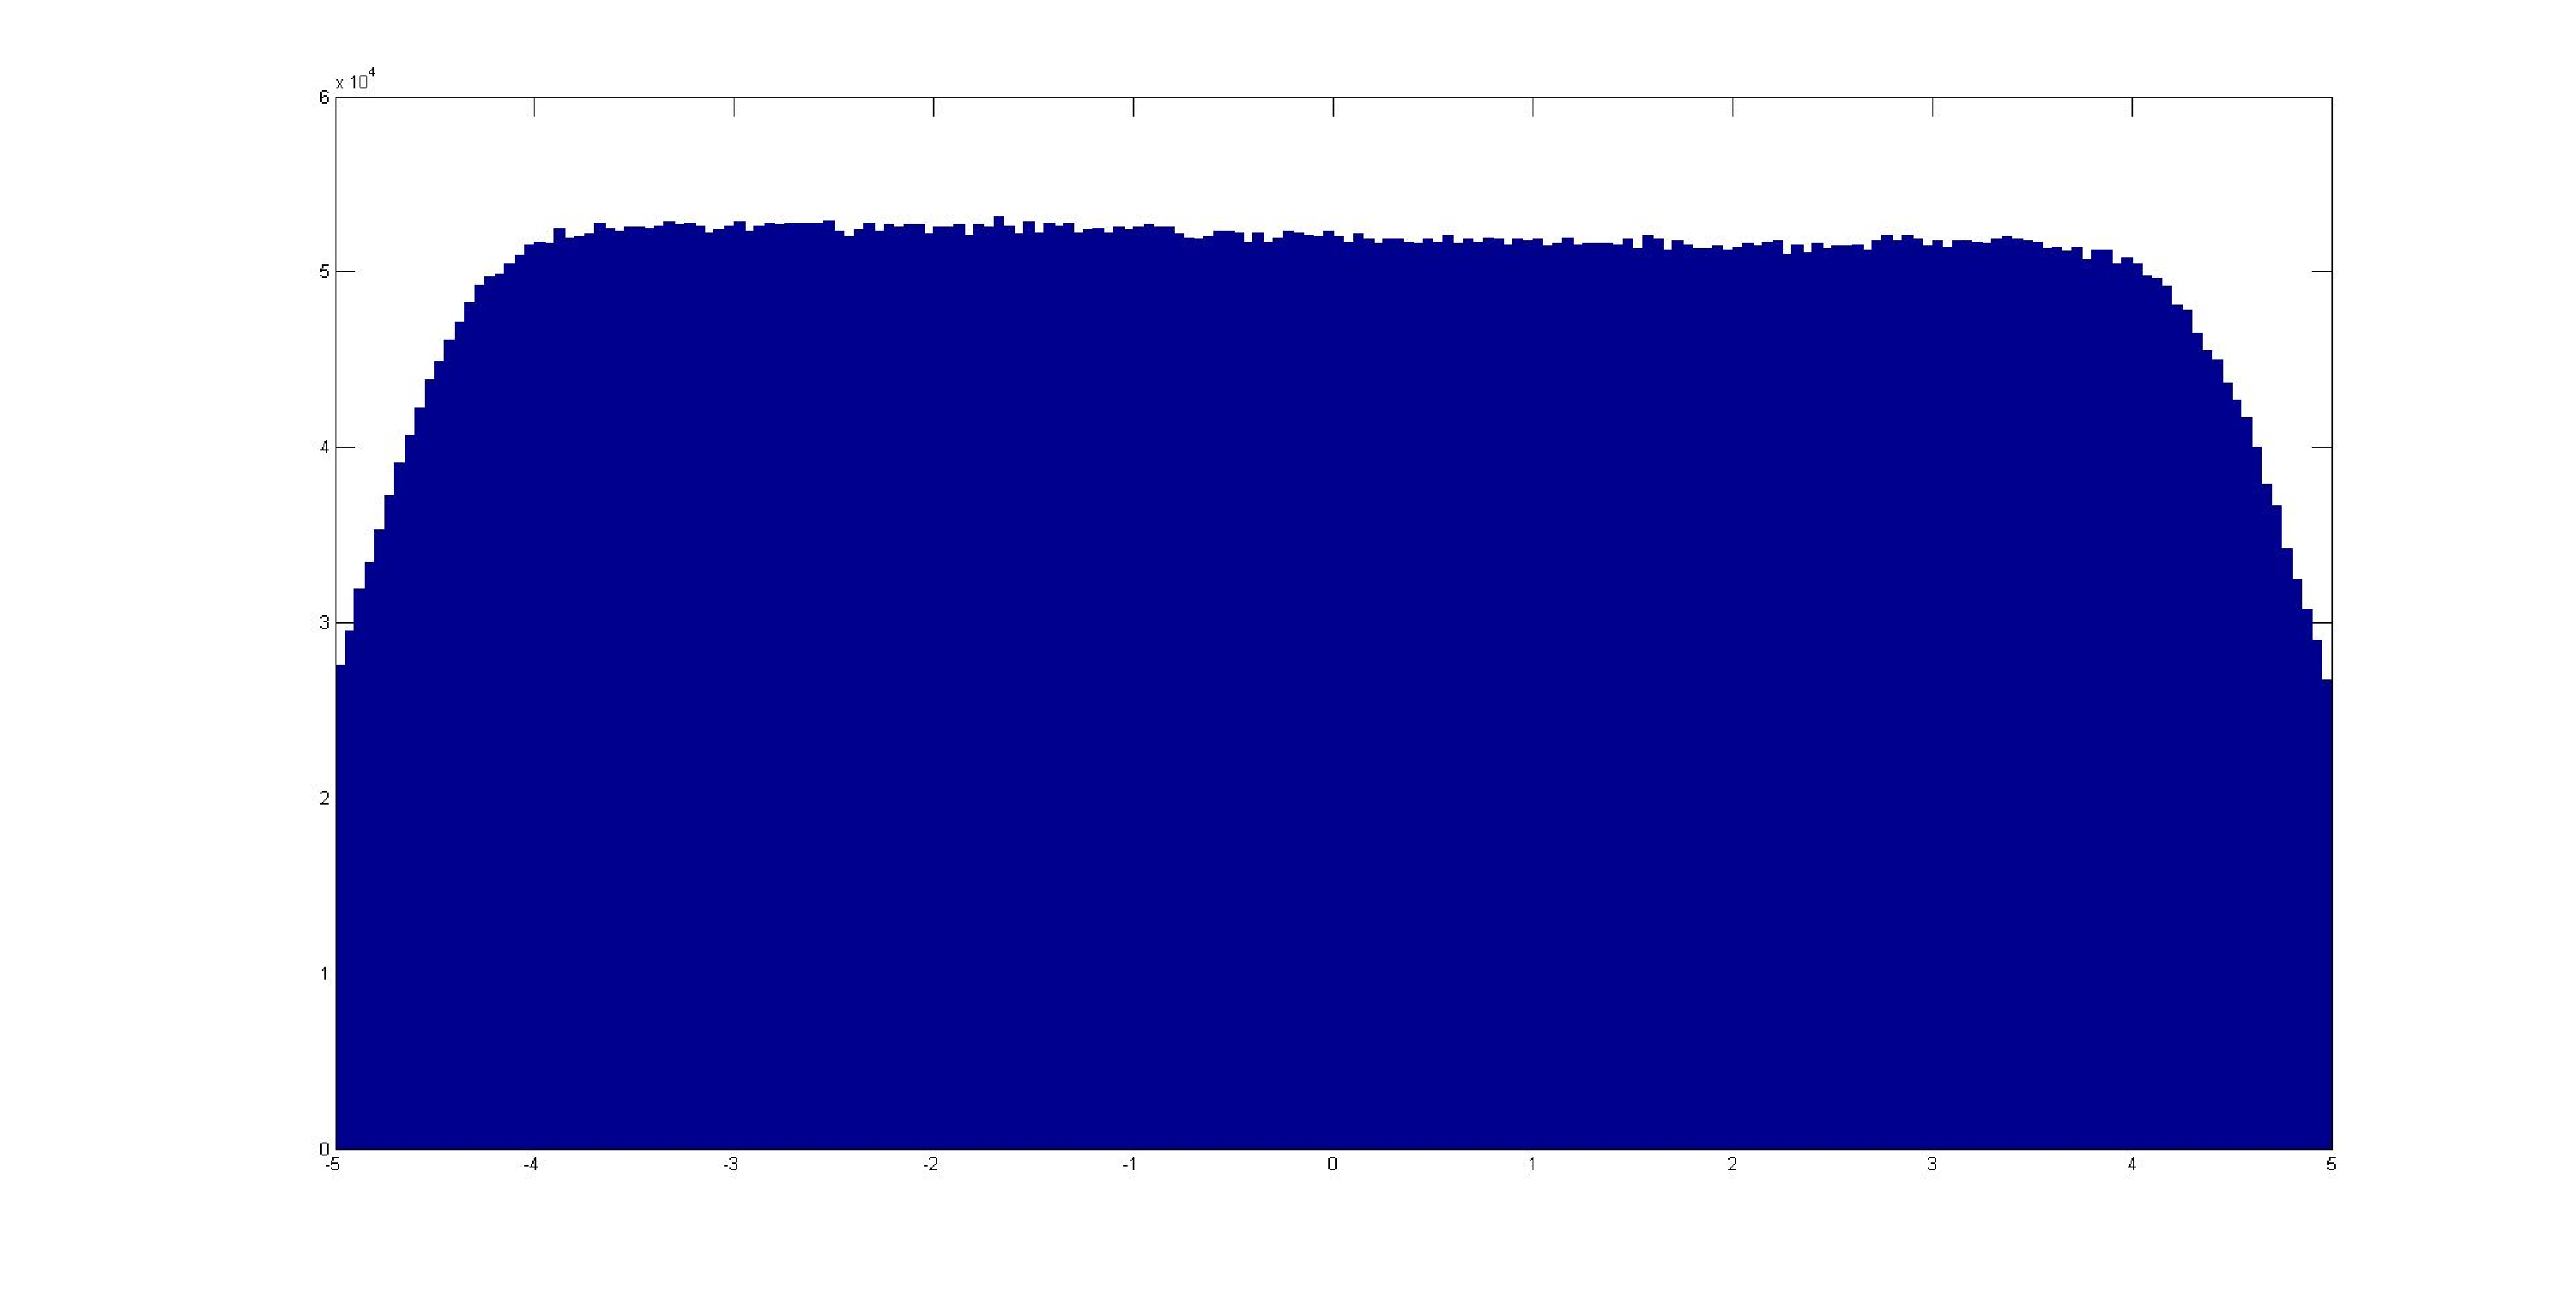
\includegraphics[width=\textwidth]{s_n_10M_1__5_5}
\caption{Rozkład normalny}
\end{figure}

\begin{figure}[H]
\centering
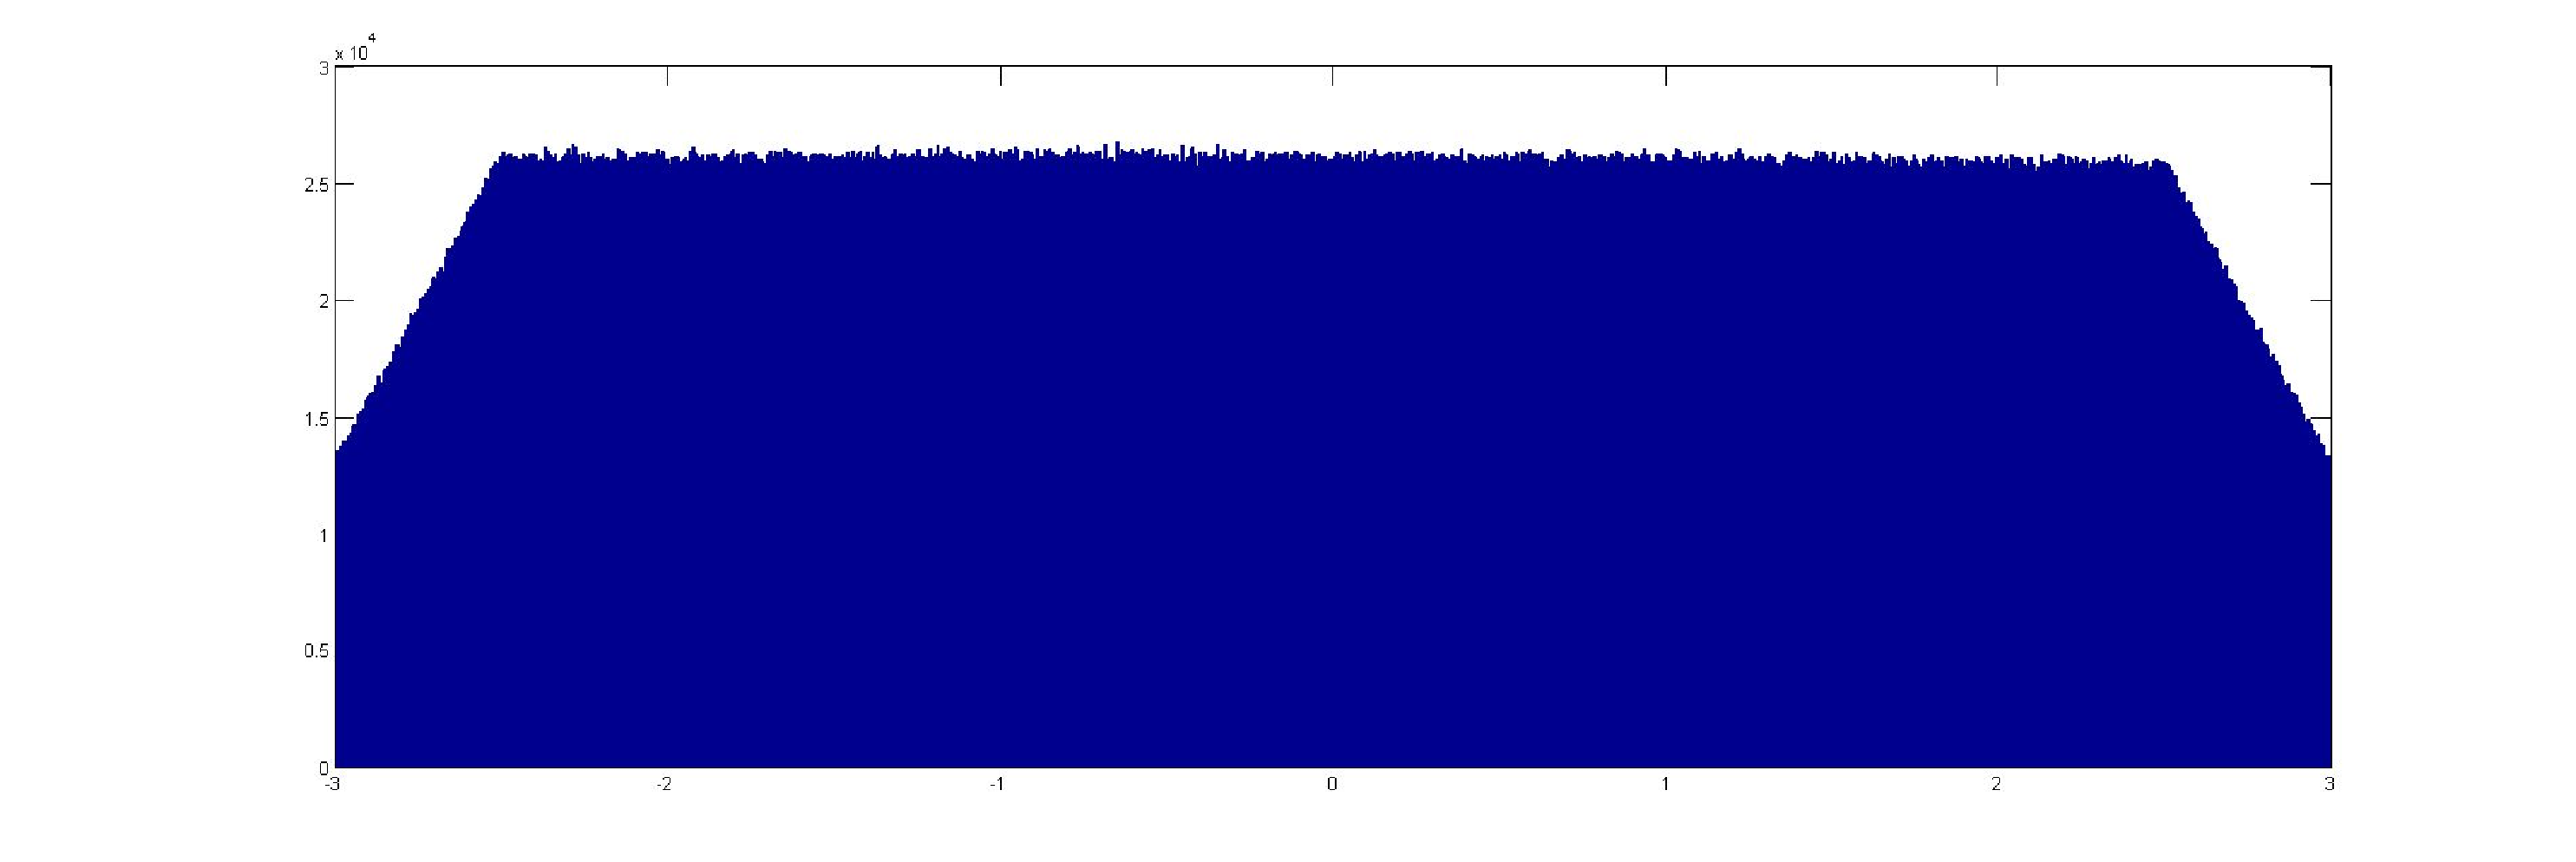
\includegraphics[width=\textwidth]{s_j_20M_1__3_3}
\caption{Rozkład jednostajny}
\label{bladzenie:probkowanie1dj}
\end{figure}

\subsubsection*{Zawijanie}
Wyobraźmy sobie, że naszą symulację przeprowadzamy bez ograniczeń, następnie naszą tniemy w równych odstępach wzdłuż każdej osi. Na koniec tak pocięte wyniki łączymy w jednym wykresie. Takie zachowanie tak naprawdę symuluje zawijanie. W związku z tym nie dziwi fakt, że poniższe histogramy przedstawkają rozkład jednostajny z szumem.
\begin{figure}[H]
\centering
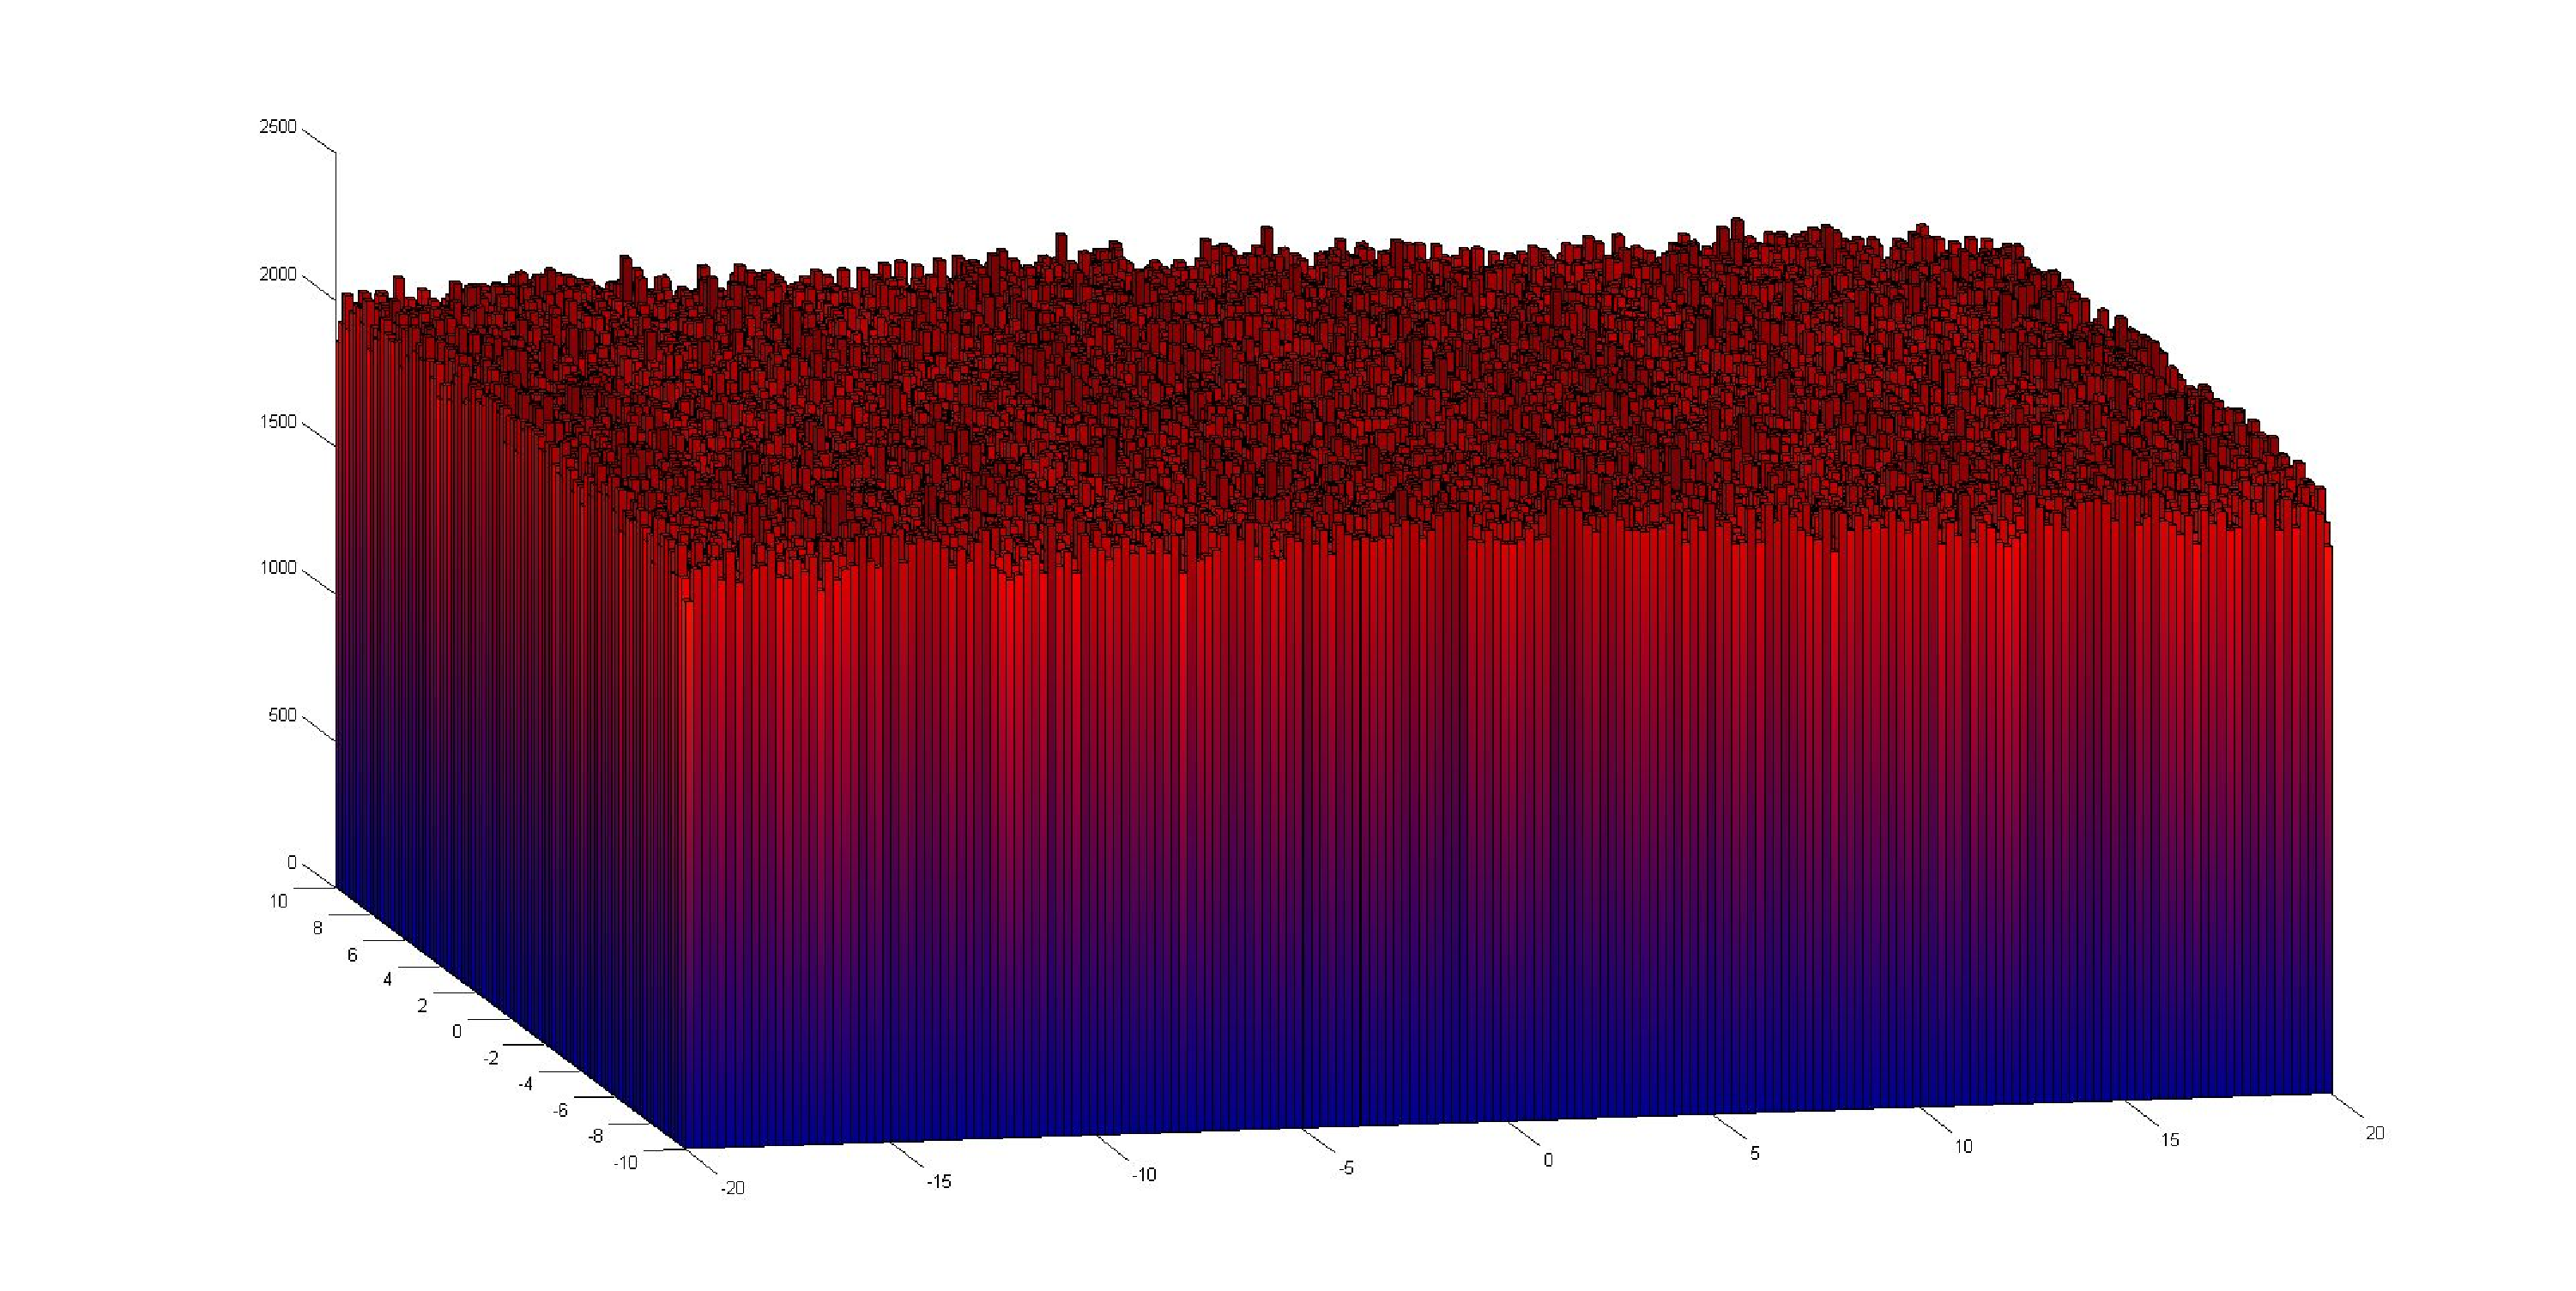
\includegraphics[width=\textwidth]{w_n_10M_2__20_20__10_10_4_2}
\caption{Rozkład normalny na dwóch wymiarach z kopiowaniem symetrycznym}
\end{figure}

\begin{figure}[H]
\centering
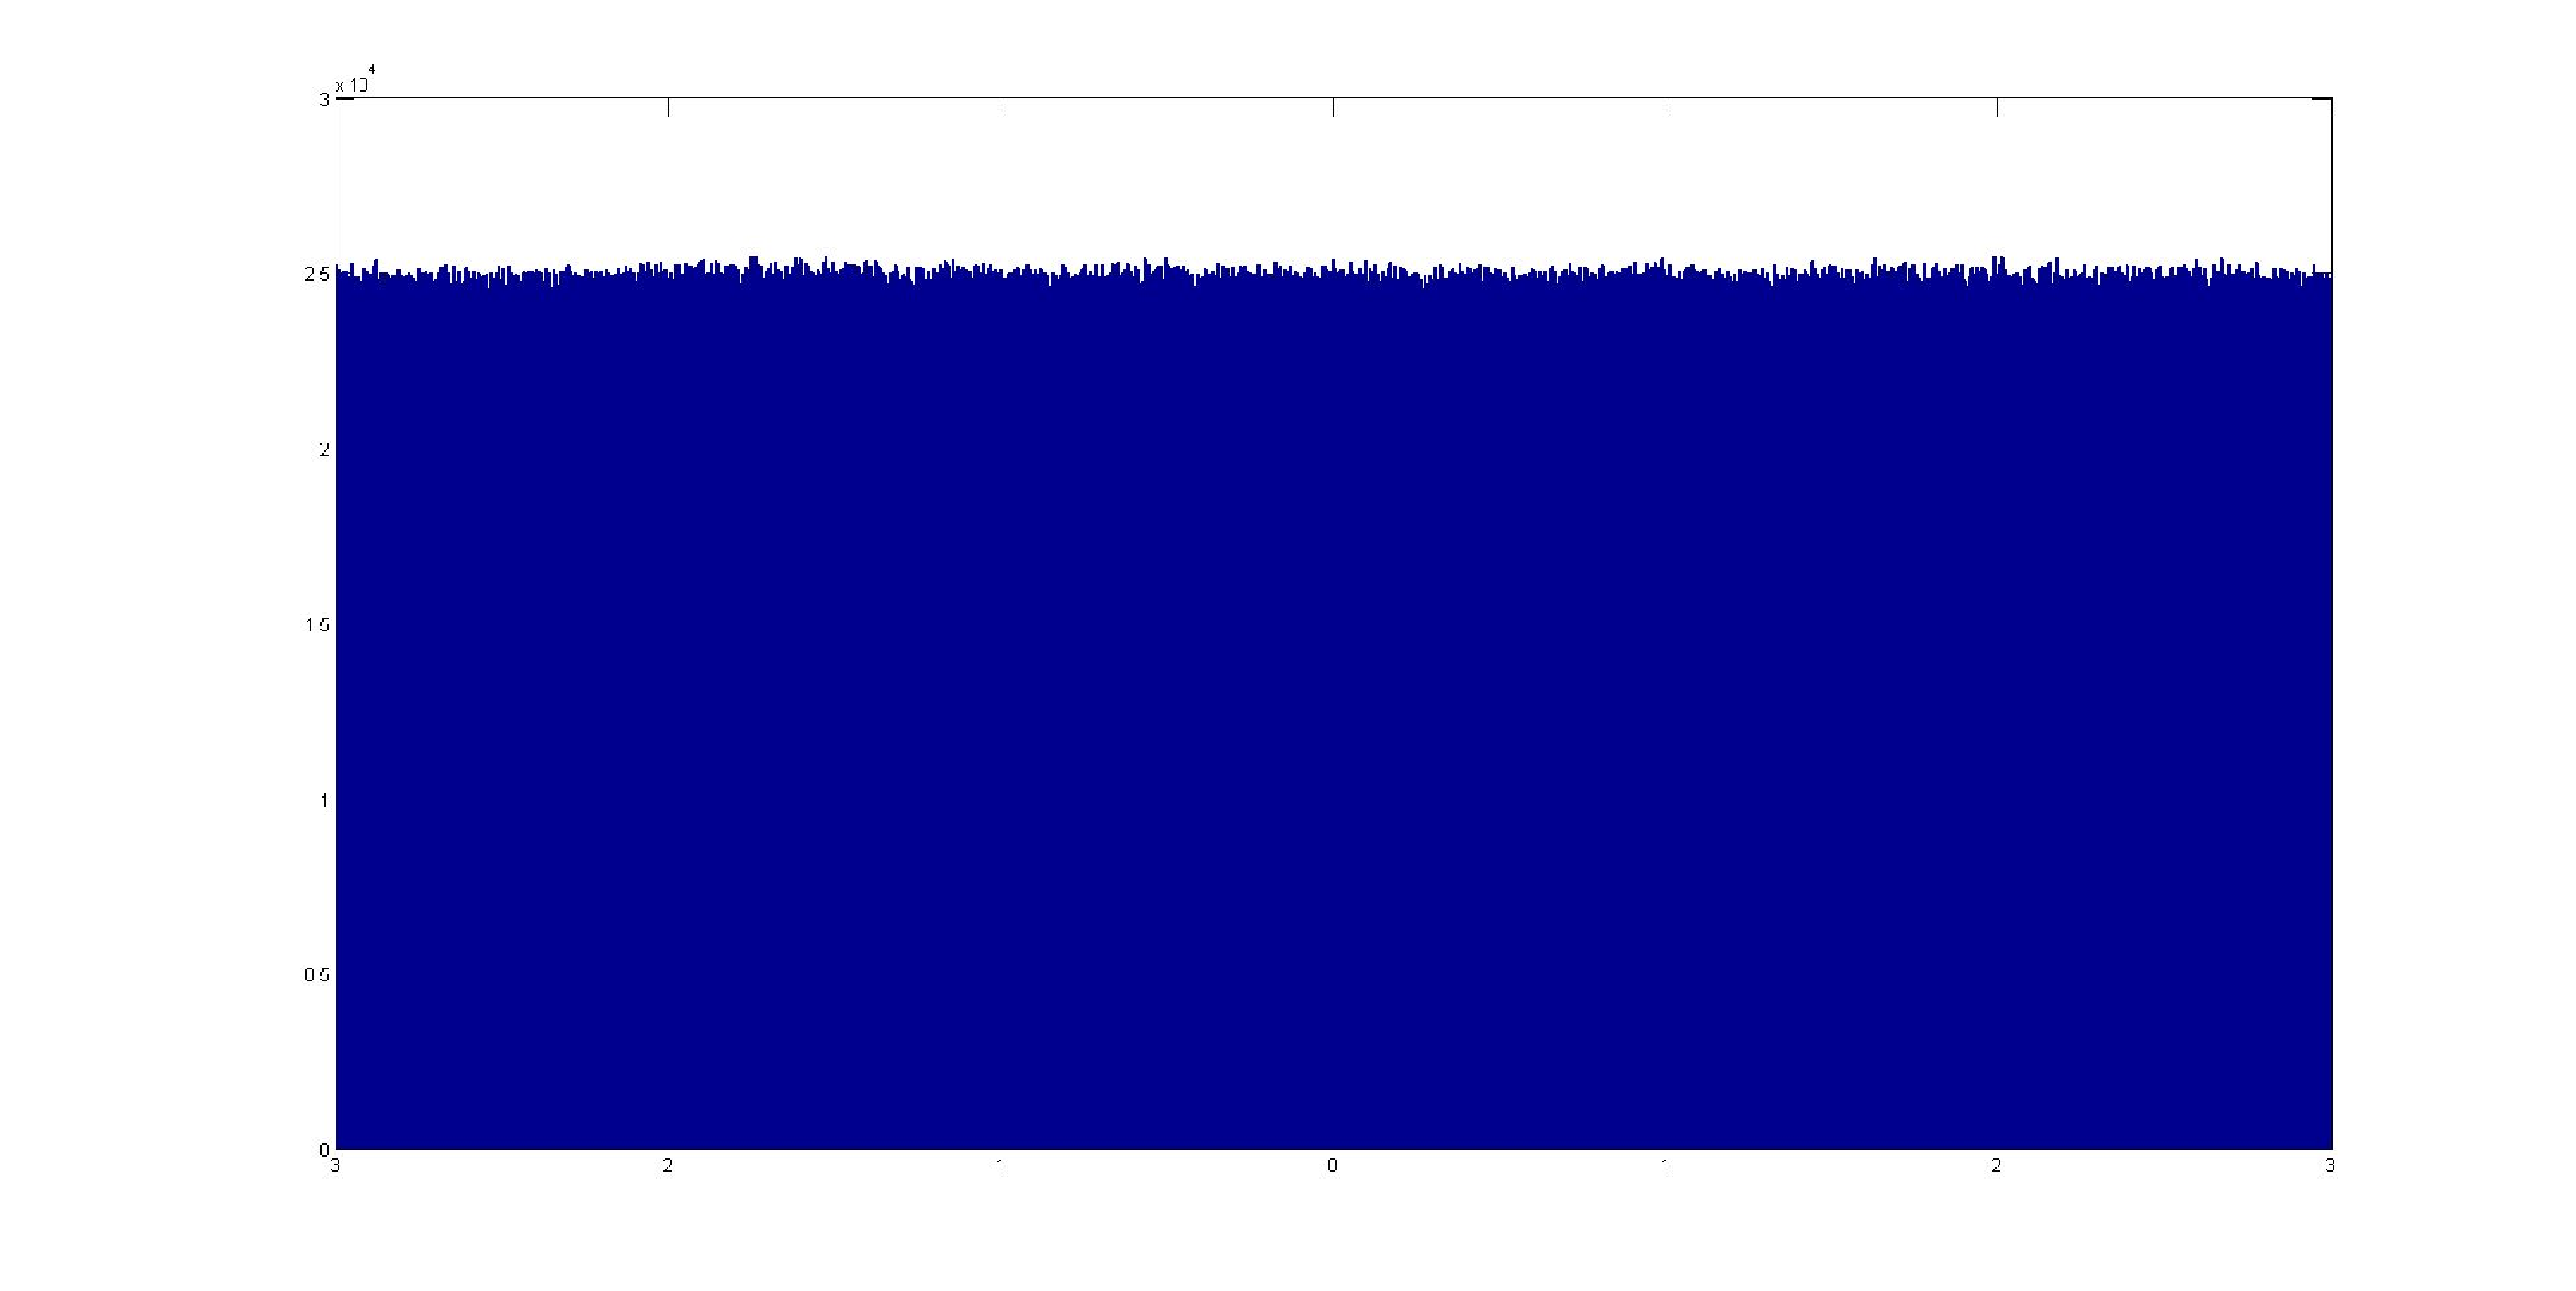
\includegraphics[width=\textwidth]{w_j_20M_1__3_3}
\caption{Rozkład jednostajny}
\end{figure}

\subsubsection*{Odbicie}
Podobnie jak zawijanie, odbicie zwraca histogram rozkładu normalnego z szumem. W tej sytuacji nieco trudniej o analogię, lecz po chwili zastanowienia nie dziwi kształt poniższych wykresów.
\begin{figure}[H]
\centering
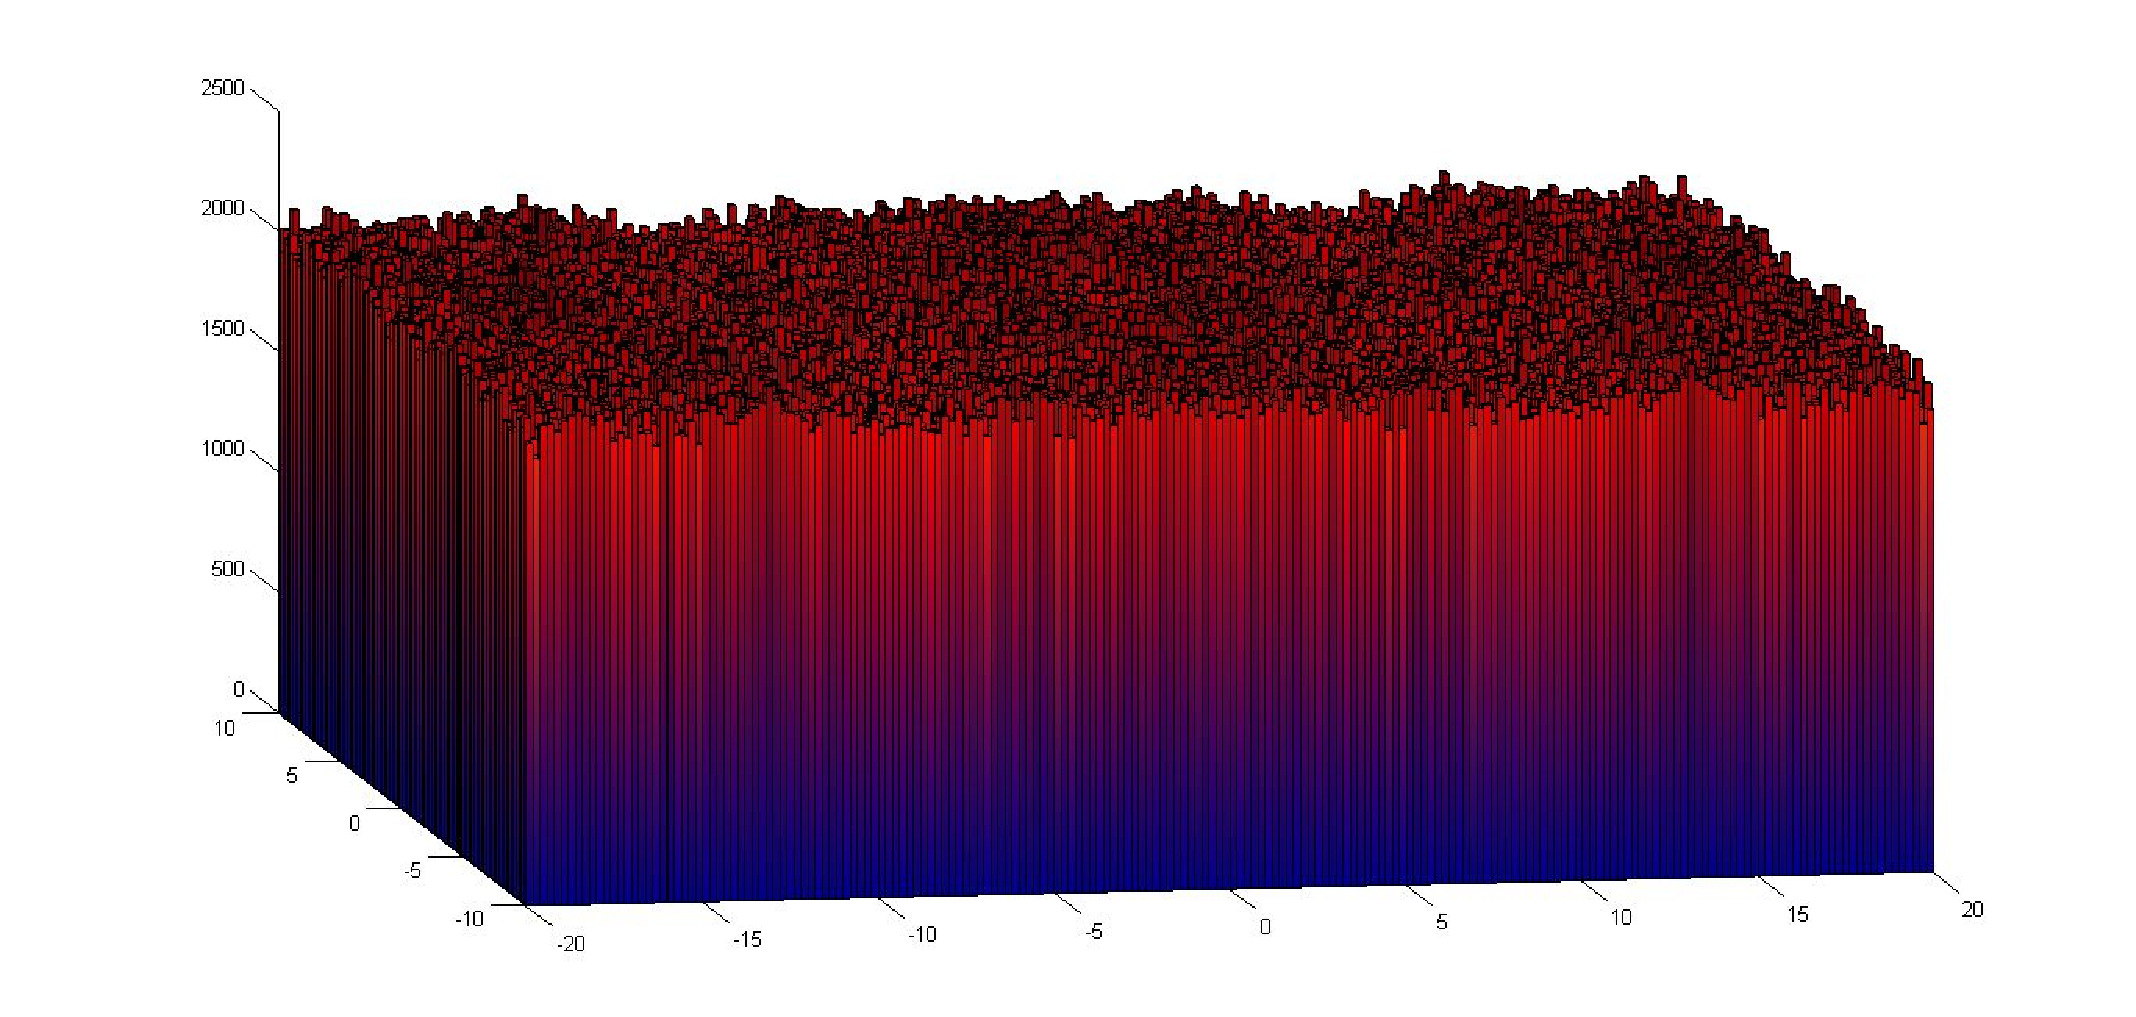
\includegraphics[width=\textwidth]{rf_n_10M_2__20_20__10_10_4_2}
\caption{Rozkład normalny na dwóch wymiarach z kopiowaniem symetrycznym}
\end{figure}

\begin{figure}[H]
\centering
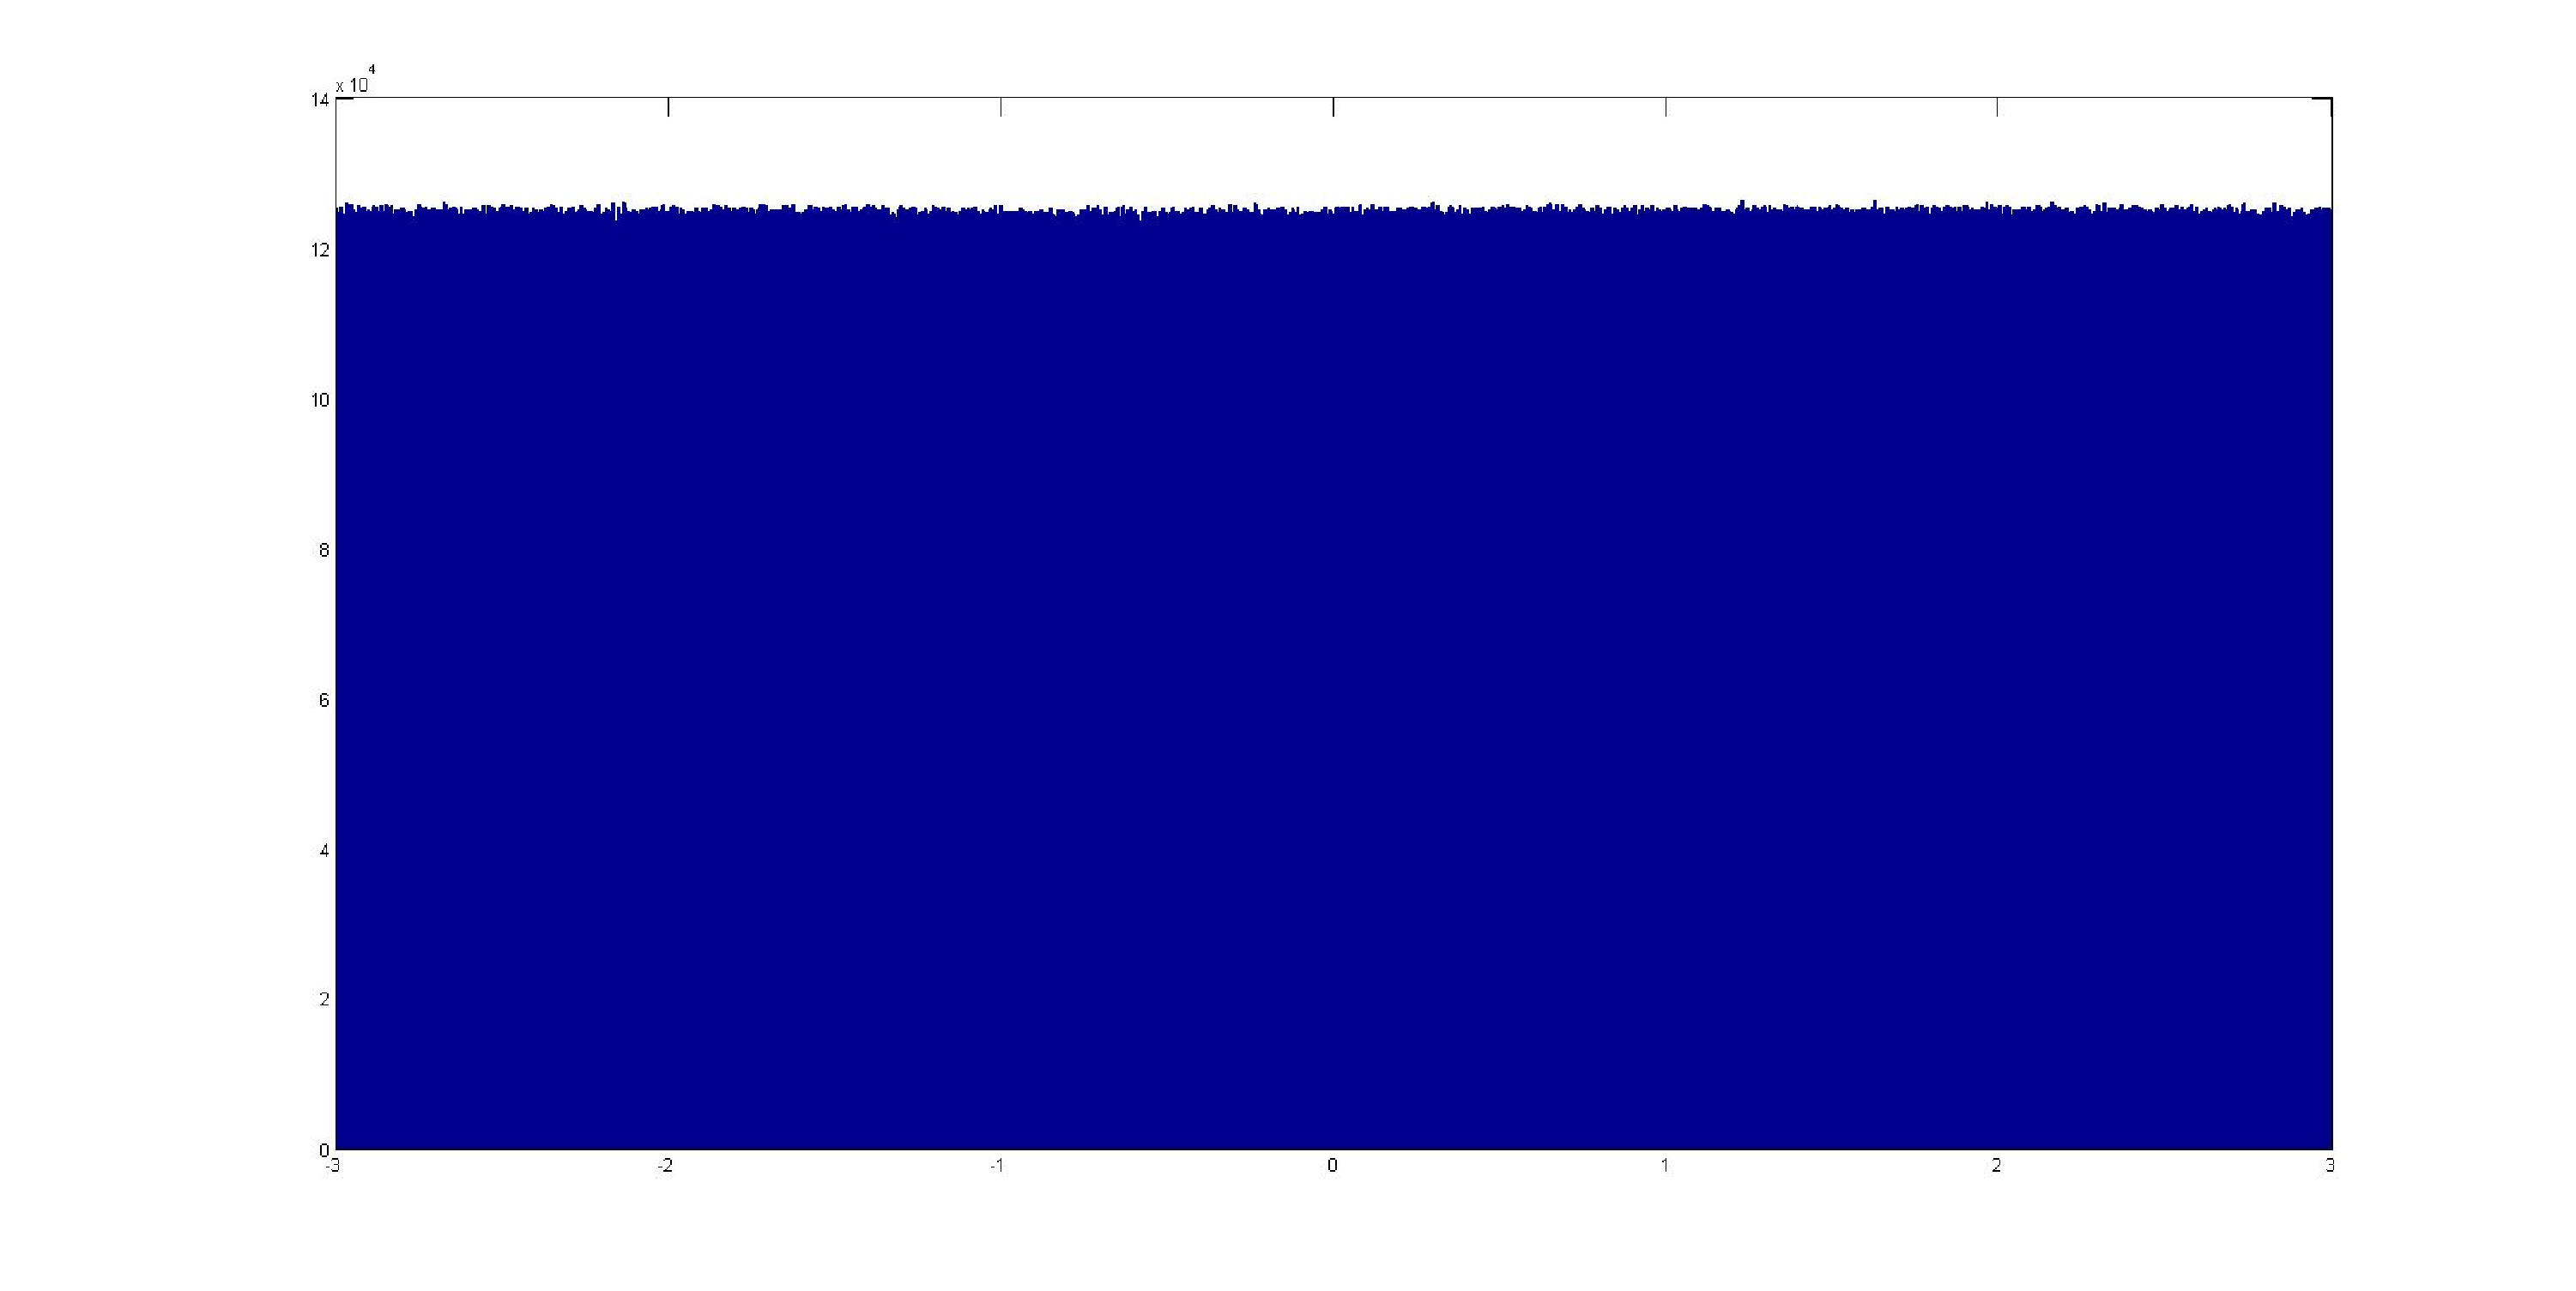
\includegraphics[width=\textwidth]{rf_j_100M_1__3_3}
\caption{Rozkład jednostajny}
\end{figure}

\begin{figure}[H]
\centering
\subfloat[test 1]{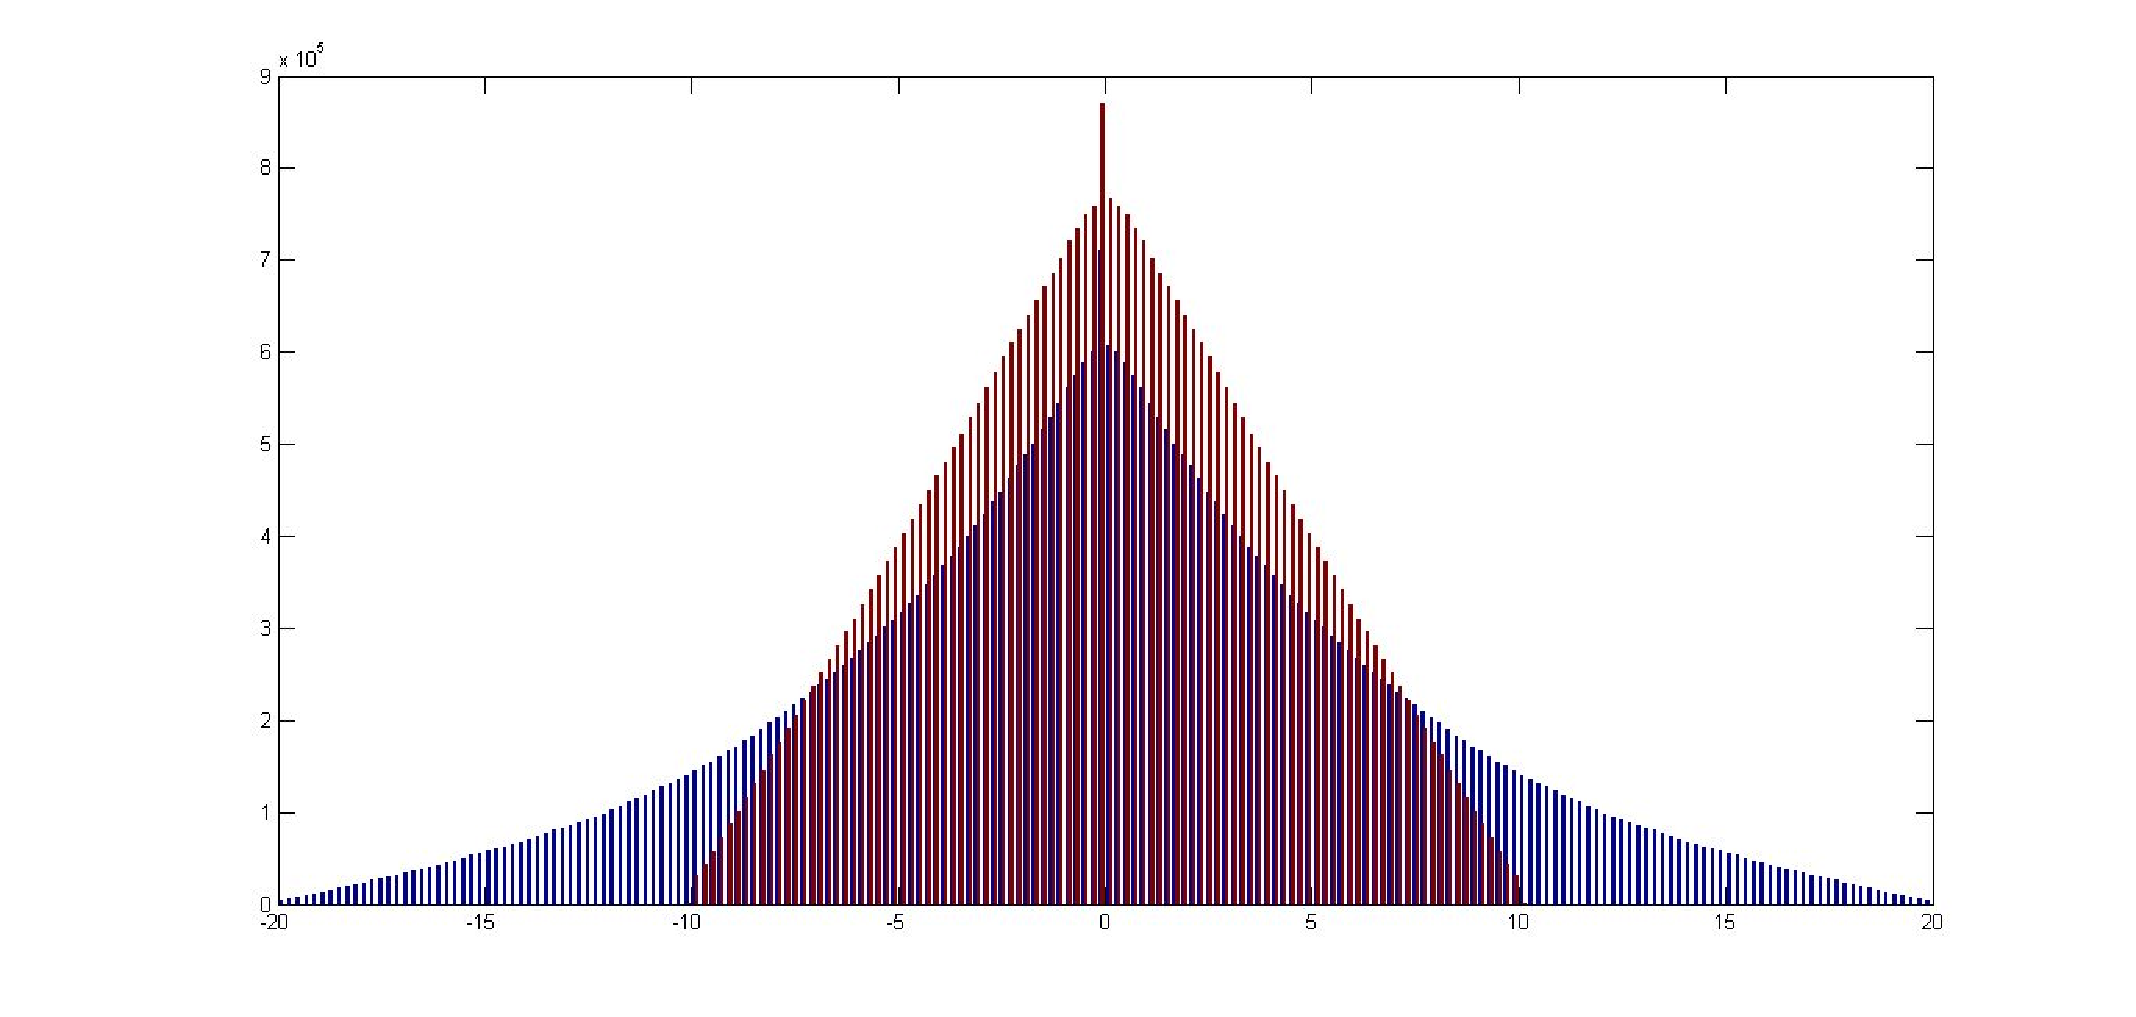
\includegraphics[width=0.45\textwidth]{ri_n_10M_2__20_20__10_10_4_1D}}
\quad
\subfloat[test 2]{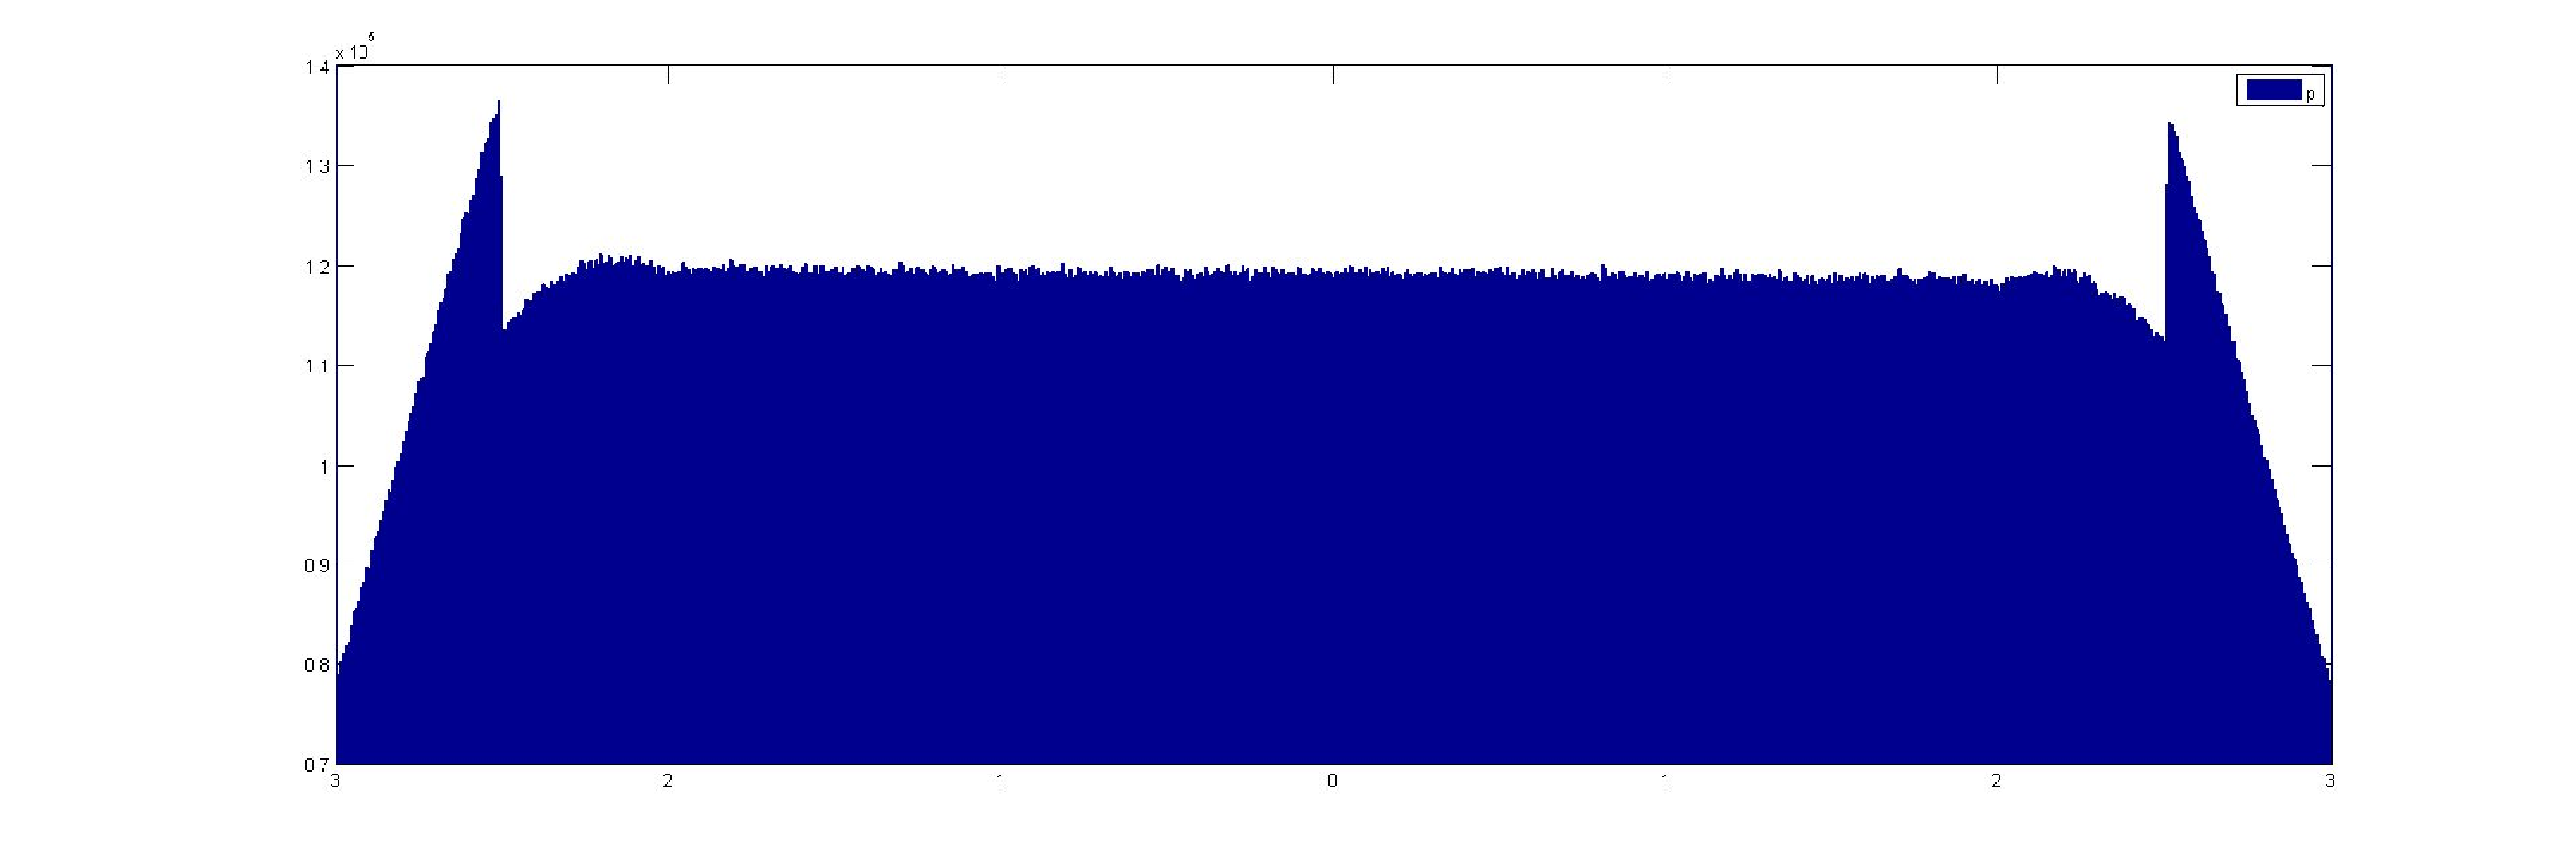
\includegraphics[width=0.45\textwidth]{p_j_100M_1__3_3}}
\caption{TEST Obrazy obok siebie}
\end{figure}

\subsection{Wnioski}

\pagebreak

\section{Benchmarki}
Zgodnie z założeniami poczynionymi w rozdziale \ref{bladzenie} testy algorytmu CMA-ES powinny przynieść rezultaty zbliżone do testów błądzenia przypadkowego.

\subsection{Metoda przeprowadzania testów}
Do przeprowadzania testów została użyta biblioteka przygotowana przez Nikolausa Hansena, współautora algorytmu CMA-ES. Podobnie, jak w przypadku błądzenia przypadkowego, wykorzystano implementację w języku MATLAB ---przypis---.

\subsection{Wnioski}

\pagebreak

\section{Wpływ technik na efektywność CMA-ES}

\subsection{Algorytm CMA-ES}
Klasyczne algorytmy ewolucyjne nie dostosowują się do charakterystyki optymalizowanej funkcji. W większości z nich rozkład prawdopodobieństwa losowanych punktów jest stały. Z tego faktu wynika problem dobrania parametrów przeszukiwania. Na przeciw tym problemom wychodzi algorytm CMA-ES, który w swej idei ma dopasowywać się do badanej funkcji.\\
Rozwinięcie akronimu CME-ES podpowiada, w jaki sposób jest to realizowane: Covariance Matrix Adaptation - Evolution Strategy (adaptacja macierzy kowariancji - strategia ewolucyjna). Punkty losowane są na podstawie macierzy kowariancji, która jest w każdej iteracji dostosowywana do aktualnej sytuacji przeszukiwań.

\subsubsection*{Szczegóły}

\pagebreak

\section{Podsumowanie}

\subsection{Wyniki}

\subsection{Możliwości rozwoju}

\pagebreak

\begin{thebibliography}{9}

\end{thebibliography}

\makestatement

\end{document}
